\documentclass[12pt,a4paper,oneside]{book}
%\documentclass[12pt,a4paper,twoside]{book} //奇数页开始

%include the configuration file for layout
%Have a look in this file it has some useful commands defined
\usepackage{setspace}
\usepackage{geometry}
\usepackage[toc,page]{appendix}
\usepackage{lipsum}
\usepackage[export]{adjustbox}
\usepackage[T1]{fontenc}
\usepackage{textcomp}
\usepackage{epsfig,graphics}
\usepackage{graphicx}
\usepackage{titlesec}
\usepackage{indentfirst}
\usepackage{verbatim}
\usepackage{fancyhdr} 
\usepackage{float}
\usepackage{amsmath}
\usepackage{hyperref}
\usepackage{xcolor}
\usepackage[nottoc,notlot,notlof]{tocbibind}
\usepackage{url}
\usepackage{algorithm}
\usepackage{algpseudocode}
%\usepackage{tabularx}
\usepackage{array}
\usepackage{makecell}
%\usepackage{tikz}
\usepackage{listings}
\usepackage{subfigure}
\usepackage{enumitem}
\usepackage[british]{babel}
\usepackage{graphicx,wrapfig,lipsum}
\fancyhf{}
\cfoot{\thepage}
\pagestyle{fancy} 


%%%%%%%%%%%%%%%%%%%%%%%%%%%%%%%%%%%%%%%%%%%%%%%%%%%%%%%%%%%%%%%%%%%%%%%%%%%%%%
% Code
%%%%%%%%%%%%%%%%%%%%%%%%%%%%%%%%%%%%%%%%%%%%%%%%%%%%%%%%%%%%%%%%%%%%%%%%%%%%%%
%New colors defined below
\definecolor{codegreen}{rgb}{0,0.6,0}
\definecolor{codegray}{rgb}{0.5,0.5,0.5}
\definecolor{codepurple}{rgb}{0.58,0,0.82}
\definecolor{backcolour}{rgb}{0.95,0.95,0.92}

%Code listing style named "mystyle"
\lstdefinestyle{mystyle}{
    frame=shadowbox, % ShadowBox
    rulesepcolor= \color{backcolour} ,
    %backgroundcolor=\color{backcolour},
    commentstyle=\color{codegreen},
    keywordstyle=\color{magenta},
    numberstyle=\tiny\color{codegray},
    stringstyle=\color{codepurple},
    basicstyle=\ttfamily\footnotesize,
    breakatwhitespace=false,         
    breaklines=true,                 
    captionpos=b,                    
    keepspaces=true,                 
    numbers=left,                    
    numbersep=5pt,                  
    showspaces=false,                
    showstringspaces=false,
    showtabs=false,                  
    tabsize=2
}
\lstset{style=mystyle}

%%%%%%%%%%%%%%%%%%%%%%%%%%%%%%%%%%%%%%%%%%%%%%%%%%%%%%%%%%%%%%%%%%%%%%%%%%%%%%
% Links
%%%%%%%%%%%%%%%%%%%%%%%%%%%%%%%%%%%%%%%%%%%%%%%%%%%%%%%%%%%%%%%%%%%%%%%%%%%%%%
\hypersetup{
    colorlinks,
    citecolor=blue,
    filecolor=blue,
    linkcolor=black,
    urlcolor=blue
}
%%%%%%%%%%%%%%%%%%%%%%%%%%%%%%%%%%%%%%%%%%%%%%%%%%%%%%%%%%%%%%%%%%%%%%%%%%%%%%
% Details of your dissertation
%%%%%%%%%%%%%%%%%%%%%%%%%%%%%%%%%%%%%%%%%%%%%%%%%%%%%%%%%%%%%%%%%%%%%%%%%%%%%%
\newcommand{\projectTitle}{Signed Distance Field Generator}
\newcommand{\fullname}{Zechen Geng}
\newcommand{\degreeTitle}{High-Performance Graphics and Games Engineering MSc}
\newcommand{\session}{2021/2022}

%%%%%%%%%%%%%%%%%%%%%%%%%%%%%%%%%%%%%%%%%%%%%%%%%%%%%%%%%%%%%%%%%%%%%%%%%%%%%%
% Change the geometry of the page to have a 25 mm binding edge
%%%%%%%%%%%%%%%%%%%%%%%%%%%%%%%%%%%%%%%%%%%%%%%%%%%%%%%%%%%%%%%%%%%%%%%%%%%%%%
 \geometry{
 a4paper,
 total={210mm,297mm},
 left=25mm,
 right=25mm,
 top=25mm,
 bottom=20mm,
 }
 
%%%%%%%%%%%%%%%%%%%%%%%%%%%%%%%%%%%%%%%%%%%%%%%%%%%%%%%%%%%%%%%%%%%%%%%%%%%%%%
% Commands to set the line spacing
%%%%%%%%%%%%%%%%%%%%%%%%%%%%%%%%%%%%%%%%%%%%%%%%%%%%%%%%%%%%%%%%%%%%%%%%%%%%%%
 %\singlespacing
 \onehalfspacing
 %\doublespacing
 
%%%%%%%%%%%%%%%%%%%%%%%%%%%%%%%%%%%%%%%%%%%%%%%%%%%%%%%%%%%%%%%%%%%%%%%%%%%%%%
% Spacing for the chapter header
%%%%%%%%%%%%%%%%%%%%%%%%%%%%%%%%%%%%%%%%%%%%%%%%%%%%%%%%%%%%%%%%%%%%%%%%%%%%%%
 \titleformat{\chapter}[display]
    {\normalfont\Huge\bfseries}{\vspace*{-1\baselineskip}\chaptertitlename\ \thechapter}{15pt}{\huge}
\titlespacing*{\chapter}{0pt}{0pt}{15pt}

\renewcommand\bibname{References}

%%%%%%%%%%%%%%%%%%%%%%%%%%%%%%%%%%%%%%%%%%%%%%%%%%%%%%%%%%%%%%%%%%%%%%%%%%%%%%
% Some shortcuts that maybe useful
%%%%%%%%%%%%%%%%%%%%%%%%%%%%%%%%%%%%%%%%%%%%%%%%%%%%%%%%%%%%%%%%%%%%%%%%%%%%%%
\DeclareTextCommandDefault{\textcopyright}{\textcircled{c}}
 
%%%%%%%%%%%%%%%%%%%%%%%%%%%%%%%%%%%%%%%%%%%%%%%%%%%%%%%%%%%%%%%%%%%%%%%%%%%%%%
% Bibliography style: choose one and make sure you have the relevant .bst file
%%%%%%%%%%%%%%%%%%%%%%%%%%%%%%%%%%%%%%%%%%%%%%%%%%%%%%%%%%%%%%%%%%%%%%%%%%%%%%
\bibliographystyle{abbrv}


%%%%%%%%%%%%%%%%%%%%%%%%%%%%%%%%%%%%%%%%%%%%%%%%%%%%%%%%%%%%%%%%%%%%%%%%%%%%%%
% Layout for the front cover !!!!! YOU SHOULD NOT HAVE TO CHANGE THIS!!!!!
%%%%%%%%%%%%%%%%%%%%%%%%%%%%%%%%%%%%%%%%%%%%%%%%%%%%%%%%%%%%%%%%%%%%%%%%%%%%%%
 
\newcommand{\frontcover}{
% The title page:
\begin{titlepage}
\newgeometry{left=25mm,right=25mm,top=45mm,bottom=0.1cm}

\begin{minipage}[t]{7cm}
\noindent\textbf{\Large{School of Computing}}\\
{\fontfamily{ptm}\selectfont 
\uppercase{faculty of engineering}
}
\end{minipage}
\hfill
\begin{minipage}[t]{7cm}
\vspace*{-25pt}

\includegraphics[scale=0.2,right]{logo_black.png}
\vspace*{-1pt}
\end{minipage}

\noindent\makebox[\linewidth]{\rule{\paperwidth}{0.4pt}}

\centering
\vspace*{37mm}
\textbf{\Large\projectTitle}\\
\vspace*{10mm}
\textbf{\large\fullname}\\
\vspace*{10mm}
\textbf{Submitted in accordance with the requirements for the degree of}\\
\textbf{\degreeTitle}\\
\vspace*{10mm}
\session\\
\restoregeometry
\end{titlepage}
}

%%%%%%%%%%%%%%%%%%%%%%%%%%%%%%%%%%%%%%%%%%%%%%%%%%%%%%%%%%%%%%%%%%%%%%%%%%%%%%
% Define a new environment for the dissertation summary
%%%%%%%%%%%%%%%%%%%%%%%%%%%%%%%%%%%%%%%%%%%%%%%%%%%%%%%%%%%%%%%%%%%%%%%%%%%%%%
\newenvironment{dissertationsummary}
 	{\cleardoublepage \null 
 		\begin{center}%
			\textbf{Summary}
		\end{center}}%
	{\vfill \null }


\setcounter{secnumdepth}{3}



% -----------allow algorithm cross pages-------------
\makeatletter
\newenvironment{breakablealgorithm}
  {% \begin{breakablealgorithm}
   \begin{center}
     \refstepcounter{algorithm}% New algorithm
     \hrule height.8pt depth0pt \kern2pt% \@fs@pre for \@fs@ruled
     \renewcommand{\caption}[2][\relax]{% Make a new \caption
       {\raggedright\textbf{\ALG@name~\thealgorithm} ##2\par}%
       \ifx\relax##1\relax % #1 is \relax
         \addcontentsline{loa}{algorithm}{\protect\numberline{\thealgorithm}##2}%
       \else % #1 is not \relax
         \addcontentsline{loa}{algorithm}{\protect\numberline{\thealgorithm}##1}%
       \fi
       \kern2pt\hrule\kern2pt
     }
  }{% \end{breakablealgorithm}
     \kern2pt\hrule\relax% \@fs@post for \@fs@ruled
   \end{center}
  }
\makeatother

\begin{document}
%The prelude is everything upto the start of chapter 1
\pagenumbering{roman}
\frontcover

\clearpage
\noindent The candidate confirms that the following have been submitted.\\
\begin{table}[ht!]
\begin{tabular}{|p{0.29\textwidth}|p{0.29\textwidth}|p{0.42\textwidth}|}
\hline 
Items & Format & Recipient(s) and Date \\ 
\hline 
Project Report & Report & SSO (12/08/22) \\ 
\hline
Source Code & \href{https://github.com/Strive12138/SDFProject}{GitHub Repository}& Supervisor, Assessor (12/08/22)\\

\hline
\end{tabular} 
\end{table}

\noindent Type of project: \underline{Exploratory Software}
\vspace{\fill}\\
\noindent The candidate confirms that the work submitted is their own and the appropriate credit has been given where reference has been made to the work of others.
\vspace{\fill}\\
\noindent I understand that failure to attribute material which is obtained from another source may be considered as plagiarism.
\vspace{\fill}\\
\flushright(Signature of Student)

\includegraphics[scale=0.4,right]{Images/Other/sign_Zec.png}
\rule{50mm}{1pt}
\flushleft
\vspace{\fill}
\textcopyright~\session~The University of Leeds and~\fullname
% Summary

\begin{dissertationsummary}
In recent years, signed distance field (SDF) technology has developed in the computer graphic industry. The value of this technology has been proven in many fields, including ray-marching, soft shadow and collision detection. Besides, SDF has been applied to successful commercial game engines like Unreal and film special effects software like Houdini. 

\hspace*{\fill}

This project aims to implement an application which generates the SDF for 3D models through modern Graphic API. The understanding of SDF will be acquired and enhanced during the implementation process. This report covers a brief introduction of SDF, the reason for chosen technologies and the details of implementation and evaluation, which is vital for explaining existing functionality and possible future software refactoring.
\end{dissertationsummary}

\clearpage
\centering\textbf{Acknowledgements}
\flushleft
First and foremost, I would like to thank Dr Hamish Carr, who provided valuable knowledge of geometry processing in the past year. During the process of this project, his suggestions helped me to achieve the targets correctly and quickly. I also want to thank Dr He Wang and Professor Markus Billeter for supporting and providing straightforward and valuable advice to me on academic writing.

% The contents
\tableofcontents

% The list of figures and tables Uncomments the 3 following lines
%to see a list of tables and list of figures.
%\clearpage
%\listoffigures
%\listoftables

\pagenumbering{arabic}

%include as many chapters as you have.
%the chapters are in a directory called Chapters
\chapter{Introduction}
\label{chapter1}
\section{Context}
The signed distance field (SDF) is a solution for solving boundary problems. The research of SDF in Computer Graphics, especially for 3D shapes representation, has developed \cite{SDFSurvey}. For example, collision detection \cite{RigidDetec} \cite{SoftDetec}, liquid simulation \cite{liquid} and ray-marching \cite{hart1996sphere}. In recent years, related research results have been applied in the industry, for example, the Unreal Engine \cite{uesdf}.

\section{Project Aim}

The main aim of this project is to build a tool to generate a signed distance field (SDF) for three-dimensional objects and implement a suitable SDF generate algorithm. The tool is expected to visualize the SDF calculate result as well.

\section{Objectives}

\begin{itemize}
    \item Build a application that can read in and visualize given triangular meshes.
    \item Implement a SDF generating algorithm.
    \item Build a application to visualize the SDF compute result
    \item Comment the code properly for potential reuse
    \item Test the tool on multiple devices
\end{itemize}

\section{Deliverables}

\begin{itemize}
    \item A application that generate Signed Distance Field.
    \item A GitHub repository that contains the source code of the tool.
    \item The MSc project report
\end{itemize}

\clearpage

\section{Project Plan}

The project will be implemented through the waterfall model as it has precise requirements and is easy to implement \cite{balaji2012waterfall}. Every new feature will be implemented after the last phase is completely finished. The first phase is research and design. It takes four months to ensure that this project's requirement is rational and realistic. The programming work starts from the middle of June to early August. Most time is assigned to algorithm implementation, and then most time will be used to evaluate and write the report.

\hspace*{\fill}

The Gannt chart of time management for this project is shown in figure \ref{inro:gannt}.

\begin{figure}[htbp]
    \centering
    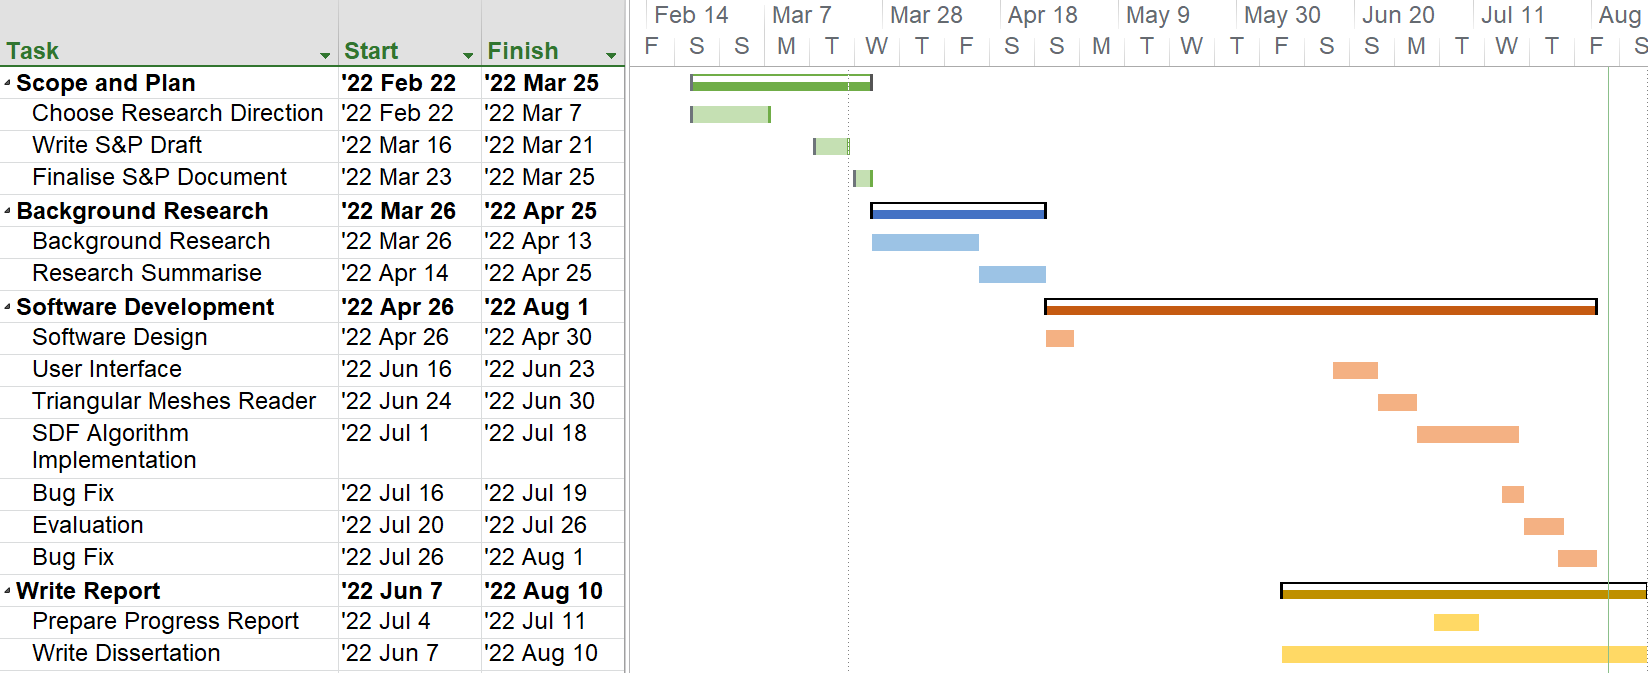
\includegraphics[width=16cm]{Images/Chap1/Gannt.png}
    \caption{The time management Gannt chart}
    \label{inro:gannt}
\end{figure}

\section{Report Structure}
This report is divided into six chapters.

\hspace*{\fill}

The first chapter introduces the project aims and objectives and discusses potential ethical, legal and social issues. The second one presents the background research for the project, including a survey of past SDF-related research and the methodology and technologies used in the project. The third chapter documents the design of the software product, while the fourth one is about detailed implementation. The contents of chapter five illustrate the test and evaluation results. Finally, the conclusion and potential improvements can be found in the sixth chapter.

\clearpage

\section{Ethical, legal, and social issues}

The SDF generate software product of this project only reads in and processes triangular meshes; it does not collect personal data at any time. Therefore, there are no significant ethical or social issues.

\hspace*{\fill}

Several open source third-party libraries have been contained and invoked in the source code to save development time and use test data sets quickly. All usage of the libraries followed its licenses to avoid potential plagiarism and legal issues.
\chapter{Background Research}
\label{chapter2}

\section{Literature Survey}

\subsection{2D Distance Field}

The term "Distance Field" or "Distance Function" was first introduced by Rosenfeld and Pfaltz \cite{FirstDistancefield} in 1966, which was applied to solve digital image processing problems. Therefore, the initial research on Distance Field is related to two-dimensional image processing. 

\hspace*{\fill}

After two years of the first announcement, the distance function algorithm of Rosenfeld and Pfaltz was announced\cite{ROSENFELD196833}.
Maurer \cite{linearEDT}introduced a linear algorithm for Euclidean Distance computing, which is used to generate the Voronoi diagram. More recently, in 2007, Green \cite{Green07Fonts} from Valve shared a method of rendering anti-aliased fonts in their game product Team Fortress 2 through alpha-testing techniques. The distance function technique played a vital role in many subdivisions of image processing in the past years.

\subsection{3D Signed Distance Field}
\label{br:3dsdf}

With the development of computer graphics, the significance of three-dimensional objects increased quickly, and the distance field technique has been applied to deal with three-dimensional problems \cite{3DDFmeta} \cite{SDFSurvey}. Jones et al. \cite{SDFSurvey} have done a comprehensive review in 2006, contributing to understanding the early research of the three-dimensional distance field. In recent years, more researchers have noticed the value of SDF and explored the technology from different aspects. Most of the researches centre on finding better SDF generate methods, while some other research explored the potential enrichment of SDF for other technologies.

\hspace*{\fill}

Sanchez et al. \cite{Sanchez2012EfficientEO} compared the efficiency of SDF generation by using different optimizing strategies to build Bounding Volume Hierarchy (BVH) data structure. Besides, they also explored the acceleration performance of GPU implementation.

\hspace*{\fill}

The research by Koschier et al. \cite{hpsdf} focuses on the generation aspect. Their algorithm is able to generate more accurate and continuous SDF with lower memory costs. Besides, to prove the practicability, the authors' teams applied their method's result to complex collision detection simulation scenarios and showed satisfying performance.

\hspace*{\fill}

Bán and Valasek \cite{firstorder} have published an SDF generation algorithm called First Order in 2020, which used first degree Taylor approximation to generate a signed distance field. As they proved, their method can reduce storage consumption and improve rendering efficiency while maintaining accuracy. Besides, the approximation solution may be able to be used on other functions.

\hspace*{\fill}

Meshed reconstruction is also a vital application of SDF, and several research papers discussed this direction.

\hspace*{\fill}

The research of Barill et al. \cite{windingnumber} discussed the significance of winding number for solving the fundamental problem of whether a point is the interior or exterior of a three-dimensional object. They explored a fast algorithm to test points through the winding numbers for triangle soups or point clouds. As they proved, generating signed distance field for soups and point clouds became possible by using their method, while the same problem is recognized as complicated to implement in the past.

\hspace*{\fill}

Combining the deep learning technique with 3D shape reconstruction is a new potential research orientation for computer graphics. Park et al. \cite{park2019deepsdf} introduced a learning reconstruction method named DeepSDF. The key to their solution is using a deep neural network to complete the learning of signed distance function from different representations like point clouds and reconstruct continuous three-dimensional surfaces through DeepSDF.

\hspace*{\fill}

Seyb et al. \cite{nlinearspheretracing} mentioned the gap of implicit representation in deformation and animation. The SDF technology helped them explore a new non-linear sphere tracing solution technique for deform modelling, which improved the performance of existing deformation techniques. Besides, they hope their research makes the industry focus on the potential of implicit representation like SDF.

\hspace*{\fill}

The signed distance field also inspires some research. For instance, the research of Sanchez \cite{convolution} mentioned the problem that the signed distance field of polygon meshes is sometimes not $ C^{1} $ continuous. They explored the convolution filtering of SDF as a new solution for modelling.

\section{Methods and Techniques}

\subsection{Signed Distance Function}
For an arbitrary point p and a three-dimensional mesh $\Sigma$ in space, the unsigned distance function of p is defined as the shortest distance from p to the mesh object, to be specific, the closest point in $\Sigma$ \cite{SDFSurvey}.

\hspace*{\fill}

The formula is as \ref{br:udf}:

\begin{equation}
    \operatorname{dist}_{\Sigma}(\mathbf{p}) = \inf _{\mathbf{x} \in \Sigma}\|\mathbf{x}-\mathbf{p}\|
    \label{br:udf}
\end{equation}

Generally, the signed distance function is used for solid meshes. Assuming that the mesh $\Sigma$ is a solid mesh $ S $, its boundary can be represented as $ \partial S $ \cite{SDFSurvey}, to represent whether the point p is inside or outside the mesh, the sign function is necessary, which is defined as \ref{br:sign}:

\begin{equation}
    \operatorname{sgn}(\mathbf{p}) = \left\{\begin{array}{cl}
        -1 & \text { if } \mathbf{p} \in S \\
        1 & \text { otherwise }
        \end{array}\right.
    \label{br:sign}
\end{equation}

Finally, the complete formula of the signed distance field is as \ref{br:sdf}:

\begin{equation}
    \mathrm{d}_{S}(\mathbf{p})=\operatorname{sgn}(\mathbf{p}) \inf _{\mathbf{x} \in \partial S}\|\mathbf{x}-\mathbf{p}\|
    \label{br:sdf}
\end{equation}

\subsection{Computing Methods of Signed Distance Fields}
\label{br:algorithm1}

Frequently, the most effective solution for three-dimensional representation is using triangular meshes. Therefore, generating a distance field for triangular meshes is a developed direction for the three-dimensional signed distance field research. For SDF generating, the mesh needs to be a closed and watertight manifold \cite{SDFSurvey}. The following discussion concentrate on this type of object.

\subsubsection{Distance Function Computation}
\label{br:dfc}

To compute a whole distance field, first, we have to solve the problem of calculating the distance from a single point to a single triangle.

\hspace*{\fill}

Jones \cite{jones19953d} has introduced two approaches to solve the problem. One is to calculate the distance from the point to its projection on the triangle plane, which can be seen as \ref{br:jonesproj}, and another is to convert the problem to a two-dimensional problem by using affine transformations.

\begin{figure}[htbp]
    \centering
    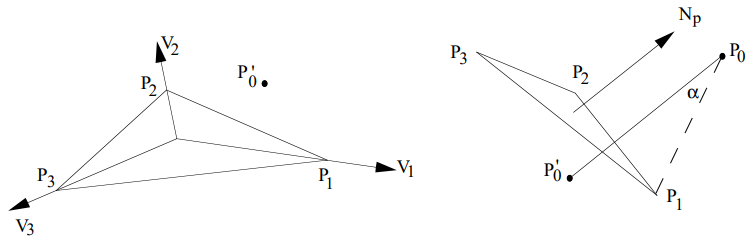
\includegraphics[width=12cm]{Images/Chap2/JonesDist.png}
    \caption{Calculating distance through projection by Jones\cite{jones19953d}}
    \label{br:jonesproj}
\end{figure}

\hspace*{\fill}

Eberly \cite{eberly2008distance} introduced a computation solution that uses the vector technique. He parameterized the triangles $ \mathbf{T}(s, t) $ as the weighted sum of two edges and a point as formula \ref{br:elberTri}:

\begin{equation}
    \mathbf{T}(s, t)=\mathbf{B}+s \mathbf{E}_{0}+t \mathbf{E}_{1}
    \label{br:elberTri}
\end{equation}

for $(s, t) \in D=\{(s, t): s \geq 0, t \geq 0, s+t \leq 1\}$, then the shortest distance can be found through calculate the minimal value of the function \ref{br:elberTriFunc}:

\begin{equation}
    \mathbf{Q}(s, t)=|\mathbf{T}(s, t)-\mathbf{P}|^{2}
    \label{br:elberTriFunc}
\end{equation}

Ericson \cite{ericson2004real} applied the Barycentric coordinates of the triangles to compute the distance. This author's method computes the distance by calculating the barycentric coordinates of point P first and then testing which Voronoi region does the projection of p located to compute the distance.

\begin{figure}[htbp]
    \centering
    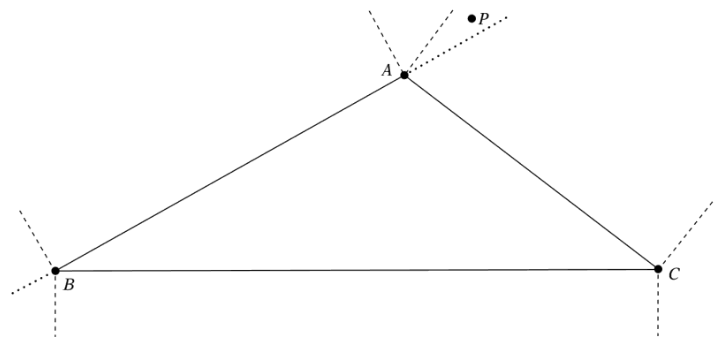
\includegraphics[width=10cm]{Images/Chap2/Barycentric.png}
    \caption{The situation of point p's projection lies on Voronoi region CA when ABC is a obtuse triangle that introduced in Ericson \cite{ericson2004real}'s paper.}
\end{figure}

Ray tracing is also a direction for solving the triangle distance problem. Tomas Akenine-M{\"o}ller and Ben Trumbore \cite{AkenineMller2005FastMS} introduced a solution which avoids pre-compute whether the ray intersects with the triangle plane. This method can compute the distance value through matrix manipulation rather than square root computation.

\subsubsection{Sign Function Computation}

Payne and Toga \cite{payne1992sdf} introduced a basic method for sign computation through scanning. The dot product of surface normal $\vec{n} $ and direction vector $ \vec{d} $ can be used to test the interior or exterior problem. However, they also noticed that this method is not always working for $ C^{1} $ discontinuous surfaces, which is the property of most polygonal meshes.

\hspace*{\fill}

An alternative is to replace the surface-normal with angle weighted pseudo-normal, which was introduced by Baerentzen and Aanaes \cite{awpseuNormal} in 2005. They first extend the angle weighted pseudo-normal of vertices introduced by Thürrner and Wüthrich\cite{awpnfirst} to edges and faces, then applied the upgraded method to the signed function computation algorithm. However, Xu and Barbi\v{c} \cite{XuagpnSlow} observed that this approach did not improve the efficiency of their research.

\hspace*{\fill}

The ray tracing method \cite{AkenineMller2005FastMS} mentioned in \ref{br:dfc} also provide a solution for testing the direction of ray and triangle intersection. If we use this method to compute the distance, then the result of normal can be reused during the sign judgement process.

\subsection{Algorithms}
\label{br:algorithm2}

After calculating the signed distance for a single triangle, the problem becomes how to compute oriental distance values for point sets.

\hspace*{\fill}

Payne and Toga \cite{payne1992sdf} introduced the naive or brutal-force method, which simply computes distances for all points in the space. The pseudo-code is shown as Algorithm \ref{br:bfalgo}:

\begin{algorithm}[H]
    \caption{Brutal Force SDF generation}
    \label{br:bfalgo}
    \begin{algorithmic}

    \For{each point(x,y,z)}
        \State $ dist=\infty $
        \For{ = each triangle t}
        \State $ newdist = distance_to_triangle(point, t) $
        \If{abs(newdist)<abs(dist)}
            \State $ dist = newdist $
        \EndIf
        \EndFor
    \EndFor

    \end{algorithmic}
\end{algorithm}

Inigo Quilez, the developer of ShaderToy \cite{shadertoy} published the SDF calculation method for most of the basic geometric shapes like Boxes and Capsules \cite{IQSDF}, but decomposing the arbitrary objects into fundamental shapes is not realistic.

\hspace*{\fill}

Both Frisken et al. \cite{frisken2000sample}, and \cite{Ju2004sample}'s researches used the sampling method to generate the signed distance without computing every triangle. For this project, it can be a potential solution. Specifically, the testing can be used through the ray intersection test. A number of equally distributed sample rays should be generated for a single sample grid to test the intersection with models. Regarding the grid as a sphere, the sample ray can be generated by dividing the sphere equally, Ahn \cite{glsphere} provided a method to calculate the coordinates of arbitrary points on the sphere by splitting the sphere. This method can be used to generate the sample rays for any direction.

\hspace*{\fill}

Building SDF for objects is time-consuming, especially when the object has a large number of triangles. Fortunately, as for a similar technique, ray tracing, the solution for the same problem has been explored for a long time and can apply to the signed distance field.

\hspace*{\fill}

To reduce the count of the traverse, we need to reduce the range of computing. Bounding volume is a widespread solution. There are several choices for constructing a bounding volume for three-dimensional meshes. The bounding sphere is the most simple choice. However, using a sphere as a bounding volume is usually unbefitting for three-dimensional objects. The distance computing through the bounding sphere contains expensive square root computation to reduce the efficiency \cite{Sanchez2012EfficientEO}. The Axis-aligned bounding box (AABB) has developed research, which is widely used for ray tracing\cite{Havran2000HeuristicRS}. This structure has a good balance of generation time and quality. Therefore, AABB is the most popular choice for acceleration \cite{Sanchez2012EfficientEO}.

 \begin{figure}[htbp]
    \centering
    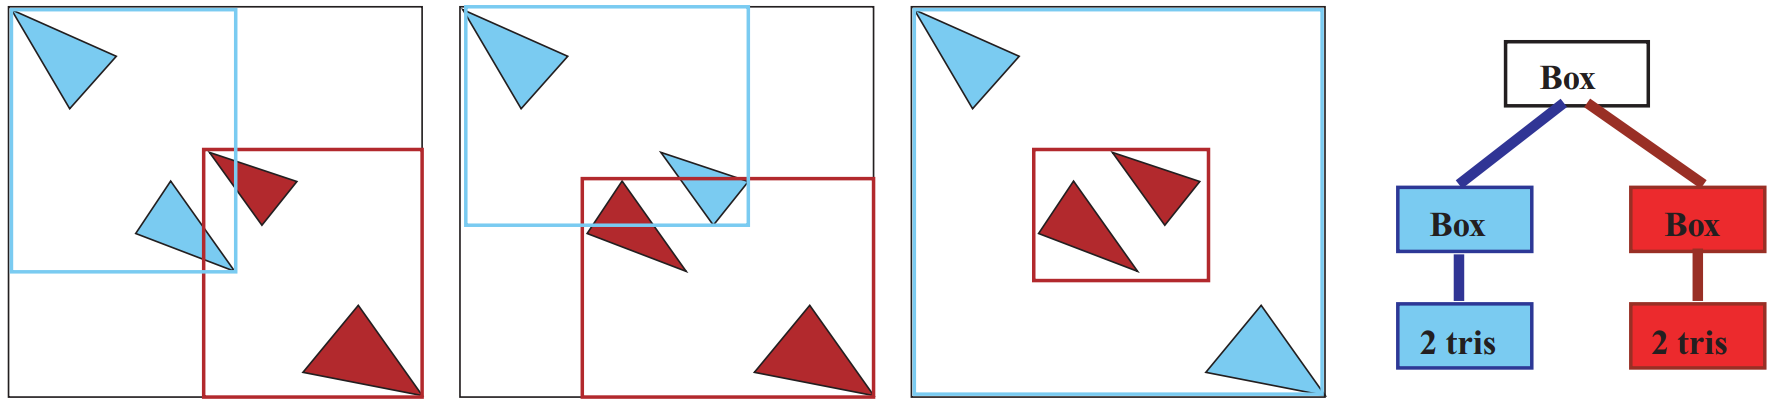
\includegraphics[width=16cm]{Images/Chap2/BVH.png}
    \caption{Different BVHs for 4 triangles provided by Wald \cite{bvhraytracing}}
    \label{br:bvh}
 \end{figure}

 Similarly, the acceleration structure for ray tracing can be extended to SDF computation. There are two primary tree-structured options: Bounding Volume Hierarchy (BVH) and K-dimensional Tree, representing two different solutions directions.

\hspace*{\fill}

 BVH split the whole object according to its primitives, for this project, triangles. Wald \cite{bvhraytracing} gives a brief explanation of BVH in his research. When building a BVH, it is recursively creating newer and smaller bounding volumes according to the size of primitives for every children node; as a result, the edge of children nodes' bounding volume can be different from its parent. Each leaf node store the bounding volume for different primitives. Ideally, different primitives will only be saved to one single leaf node and can be traversed through parent nodes. Strategies for building BVH are illustrated in figure \ref{br:bvh}.

\hspace*{\fill}

The principle of the KD-tree building is similar to BVH, except the method of splitting the space is different. The KD-tree structure is mostly built using AABB bounding volume \cite{kdraytracing}. Building a KD tree for space will recursively divide the whole space with the position of primitives alongside the axis. The bounding box of the children nodes must share some edges with its parent nodes. When ray tracing through the KD-tree structure, the algorithm will test whether the ray intersects with the bounding box. If a ray only intersects one side of a box, then the ray must shoot on a primitive contained in the box node; the traverse will continue until the correct leaf node is found \cite{kdraytracing}. In the comparison of Havran\cite{Havran2000HeuristicRS}, this structure is the best method for CPU implementation. As for SDF generation, Inigo Quilez has a WebGL implementation on ShaderToy \cite{kdtoy}, which proved that the solution fits the requirement of SDF computation. An example given by Foley \cite{kdraytracing} of KD-tree ray tracing showed in figure \ref{br:kd}. 

\begin{figure}[htbp]
    \centering
    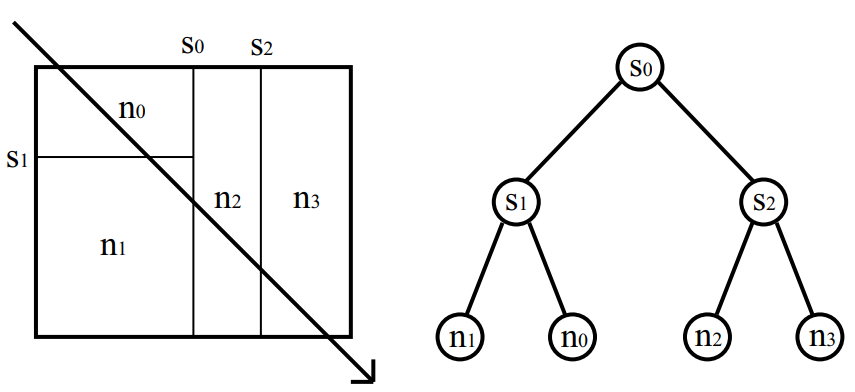
\includegraphics[width=14cm]{Images/Chap2/kd.png}
    \caption{Left: The principle of kd-tree ray tracing. Right:The structure of the same tree}
    \label{br:kd}
\end{figure}


\subsection{Technologies and Tools}
\label{br:tt}

\subsubsection{Graphics APIs}
\label{br:api}

In computer graphics, the Graphics Application Programming Interface, or Graphics API, plays a vital role in determining how the GPU manipulate the rendering tasks. For the graphics programmers, a friendly API will increase the development efficiency.

\hspace*{\fill}

Three Graphics APIs are widely used: OpenGL, Vulkan and Direct3D.

\paragraph{OpenGL}

Open Graphic Library or OpenGL \cite{OpenGLofficial}, is a cross-platform and language-independent Graphics API, which was initially developed by Silicon Graphics, Inc. (SGI) \cite{kessenich2016opengl}. Khronos Group has continued to manage the development of this API since 2006. Its Version 1.0 was released in July of 1994, and the latest version was updated to 4.6. OpenGL is able to render both 2D images, and 3D graphics through a graphics processing unit (GPU) \cite{kessenich2016opengl}. Although C++ is the most chosen programming language for developing OpenGL applications, using JavaScript, C and Java to create OpenGL applications on IOS, Android or web browsers are available.

\paragraph{Direc3D}

Direct3D \cite{d3dofficial} is the main competitor of OpenGL and Vulkan created by Microsoft. It only runs on Microsoft environments like Windows, Xbox and UWP applications. As a low-overhead Graphics API, Direct3D allows the programmer to control synchronization and multi-threading; compared with standard APIs, it has higher efficiency and saves more resources \cite{d3d10} \cite{blythe2006direct3d}.

\paragraph{Vulkan}

Vulkan is the newest Graphics API, which was developed by Khronos Group and first released in February of 2016. Vulkan was positioned as the successor of OpenGL, it keeps cross-platform capabilities and aims to create the graphic applications with complex, and numerous datasets \cite{sellers2016vulkan}. Therefore, Vulkan will be widely used in industry in the future. Vulkan gives the programmer a high degree of freedom during the development process; the responsibility of synchronization, scheduling or memory management and many other features belongs to the programmer, which also means that compared with OpenGL, Vulkan gives higher requirements on the experience for application writers \cite{sellers2016vulkan}.

\subsubsection{Languages}

\paragraph{C++}

C++ is a general-purpose programming language based on the C programming language \cite{c++iso}, developed by Bjarne Stroustrup and released in 1985 \cite{Stroustrup1997}. C++ is widely used in the graphics industry. All of the Graphics APIs mentioned in \ref{br:api} provide support for C++, and Vulkan only officially provides C++ wrapper support since the property of memory management.

\paragraph{Python}

Python \cite{pythonoffcial} is a popular interpreted, general-purpose programming language developed by Guido van Rossum around 1990 \cite{lutz2001programming}. With the development of deep learning, many popular and friendly python frameworks and libraries have been created. For example, TensorFlow \cite{TensorFlow} and Keras \cite{Keras}. There are already successful examples applying Deep Learning technology to graphics like NVIDIA's DLSS (Deep Learning Super Sampling) \cite{DLSS}. Moreover, as mentioned in \ref{br:3dsdf}, the research of Park \cite{park2019deepsdf} about signed distance field was based on deep learning technology.

\subsubsection{Graphical User Interface libraries}

\paragraph{GLFW}

GLFW \cite{glfw} is a cross-platform C library for OpenGL, OpenGL ES and Vulkan. This library allows programmers to create and handle application windows, contexts and surfaces, user input and many other functions.

\paragraph{ImGui}

Dear ImGui \cite{dearimgui} is a open-source C++ graphical user interface library developed by Omar Cornut. The core source code of Dear ImGui is only contained in several platform-independent files. Therefore, it is portable and easy to be compiled with other application codes. Most of the mainstream Graphics APIs, including DirectX, OpenGL, Vulkan, and platforms including Windows, OSX are supported. Dear ImGui also provides useful extensions, including Text Editors and Animation Editors.

\paragraph{Qt}

Qt \cite{qt} is a robust cross-platform UI framework for C++ \cite{sherriff2018qt}, which was initially developed by Haavard Nord and Eirik Chambe-Eng in 1990, and the responsibility of development belongs to The Qt Company. Qt provides a series of tool kits for UI development, including declarative language QML \cite{qml}, compilation tool qmake \cite{qmake} and an integrated development environment (IDE) Qt Creator \cite{qtcreator}. The programmer is able to create a complete application only in Qt environment. 

\subsubsection{Building Project}

\paragraph{Premake}
\label{premake}

Premake \cite{premake} is open-source utility software for source code building. Lua \cite{lua} Script is used for premake to store the information of software projects. Premake use the command line to read the project configuration for different platforms from a Script and generate project of development IDEs 

\paragraph{CMake}

CMake \cite{cmake} is an open-source compiler-independent for source code building, testing and packaging. It is mostly used for C and C++ languages. A C++ compiler like MinGW is necessary for project building. CMake also supports mainstream IDEs like Visual Studio and Xcode.

\subsubsection{Model file formats}

\paragraph{OBJ}

OBJ \cite{OBJ} file is a geometry file format developed by Wavefront Technologies for its Advanced Visualizer animation tool. This format contains the positions of vertices, UV mapping information, vertex normals and the list of each polygon face. OBJ files store the information of vertex in counter-clockwise order. Wavefront Technologies also developed the Material Template Library (MTL) format for OBJ to store the material properties of objects.

\paragraph{FBX}

FBX (FilmBox) \cite{FBX} is a file format for 3D models, which was initially developed by Kaydara for MotionBuilder and owned by Autodesk in 2006. FBX file is a tree-structured document and can be used for animation by storing the motion nodes.


\section{Choice of Methods}

\subsection{Choice of Method and Algorithm}
\label{br:cAlgo}

Considering about the difficulty of implementation and time limitation, several methods and algorithms are chosen for this project. 

\hspace*{\fill}

First, the field generation method is sampling the points in a limited bounding box range and calculating the distance values for them through a number of sample rays; when setting the appropriate parameters (e.g. resolution, number of sample rays), we can get a satisfying result. Second, the chosen method of computing signed distance values is the ray tracing solution \cite{AkenineMller2005FastMS} mentioned in \ref{br:dfc}, because this method solves the distance function computation problem through matrix rather than square root computation, which will get the exact value with relatively low consumption. Then, the acceleration strategy is applied KD-tree data structure alongside the AABB bounding volume during the process of constructing the signed distance field, which is a widely used space acceleration structure; the successful commercial game engine Unreal Engine uses this structure to generate SDF \cite{uesdf}. Finally, using multi-threading programming to improve efficiency. Undoubtedly, GPU implementation is a better way for acceleration for generating SDF. However, the HPG courses are not cover related content like CUDA programming; therefore, GPU implementation will be a tricky method for this project and may result in the project not being completed on time. Besides, avoiding GPU implementation brings better compatibility since there will be no requirement for specific hardware.

\subsection{Choice of Technologies}
\label{br:ctpl}

\subsubsection{Language and Graphics API}

The libraries, frameworks and APIs mentioned in \ref{br:tt} provide support for C++. Besides, the compatibility and efficiency of C++ satisfied the requirement of Graphics application development. Therefore, C++ becomes the chosen language for this project.

\hspace*{\fill}

OpenGL and Vulkan are covered by High-Performance Graphics and Games Engineering MSc modules, while Direct3D is not. Direct3D obviously is a risky option. Besides, considering the time limitation and the requirement of Vulkan API, OpenGL becomes the final chosen API for this project because of its compatibility and relatively easy to implement.

\hspace*{\fill}

A review of the OpenGL graphics pipeline is helpful for further application design.

\hspace*{\fill}

As shown in figure \ref{br:pipeline} \cite{learopengl}, the pipeline is divided into several stages; each stage will collect the output data from its last stage and process the data for the next.

The first stage is named Vertex Specification. Two concepts should be cleared before continuing to introduce the pipeline. Vertex Buffer Objects (VBO) are the buffers containing a number of information (e.g. positions, normals, colours) of vertices in video memory \cite{vetspeci}. Vertex Array Object (VAO) contains at least one VBO as well as the definition of vertex data \cite{vetspeci}. The GPU use VAO and VBO to analyze the vertex data for rendering.

\paragraph{Vertex Shader}

Vertex Shader is a programmable stage which can be used to process the attributes of vertex \cite{vetsha}. The vertex shader is mostly used to make transformations of coordinates for vertex data, including local-world transformation, view transformation and clipping. Tessellation \cite{tesse} and Geometry Shader \cite{gs} are two optional stages; the former can divide data into smaller primitives, while the latter can modify the input to geometric shapes like triangles.

\paragraph{Primitive Assembly}

Primitive Assembly \cite{pa} aims to modify the former primitives to a sequence of basic primitives like lines. When Tessellation or Geometry Shader is active, an early primitive assembly process will happen before both \cite{vetsha}.

\paragraph{Rasterisation}

Then it comes to Rasterisation \cite{pipeall}. The output of Primitive Assembly is primitives; they will be processed to screen position by perspective and viewport transformation. The output of this stage is screen coordinates, to be specific, the position of pixels. Those pixels (fragments) will be sent to the fragment shader for colour computation in the next stage.

\paragraph{Fragment Process}

Fragment Process \cite{pipeall} is another programmable stage of the pipeline. Colours, depth values and possible stencil values will be computed in Fragment Shader \cite{fs} and set as the output of this shader, which will be passed to the final testing and blending stage \cite{psp} , where the scissor test, alpha test and depth test will happen. Finally, the data will be passed to the framebuffer and shown on the screen.

\subsubsection{GUI}

The user interface of the final application only needs a panel to show buttons, checkboxes and text information. Considering the complexity of setting up the development environment and writing Qt code, using Qt is too obese for this project. Dear ImGui is enough to implement the features mentioned above and can also avoid the potential problems caused by different Qt environments. Therefore, the project will be developed through Dear ImGui.

\hspace*{\fill}

Without Qt, the only option for application window control API is GLFW. Finally, the GUI will be created through GLFW alongside Dear ImGui.

\subsubsection{Building Project}
\label{premake2}

To generate a project through CMake, the user must install and set the appropriate environment for this tool kit. However, some potential problems will happen in specific situations, like the version differences on different devices. Compared with CMake, Premake only needs to define the configuration of the project when creating Lua script, which also enhances the understanding of project structure. Therefore, this project chose Premake as the tool for building project.

\subsubsection{Model file formats}
\label{br:cmf}

There is no requirement to make animation for the project; the OBJ file satisfies the load test models' demand and becomes the chosen format.

\subsubsection{Third Party Libraries}

Moreover, some third-party libraries help implement the application. An OpenGL Loading Library is used to load the pointers to OpenGL functions. The project chose glad \cite{glad} as the final option of this library because of a similar reason to choosing Dear ImGui. For mathematics and model load libraries, the situations are analogical; there is one widely used library for each field with no obvious alternative solutions, GLM \cite{glm} (for mathematics), and tinyobjloader \cite{objload} (for loading obj file). Therefore, they become the chosen third-party libraries.
\chapter{Software Requirements and System Design}

\section{Software Requirements}

The requirements should be defined correctly and briefly to design and implement a software product. In order to achieve this object, a detailed analysis is necessary. The following section will discuss the potential requirements from several different aspects.

\subsection{Main Function}
\label{req:main}

Initially, to figure out the requirements of a software product, the most vital work is ensuring this project's main function, or the primary target, and giving a brief description. Fortunately, the main function of this project is simple to summarise from the name, generating the signed distance field for arbitrary three-dimensional objects.

\hspace*{\fill}

Since the Wavefront OBJ has been chosen as the input file format in \ref{br:cmf}, the explanation can become more specific, generating SDF for triangular meshes. Therefore, the software is supposed to read in the data from .obj files and store the process of the information. Once the data has been stored in the memory, the software needs to analyse the data and compute signed distance functions, then store the result in a new file, and finally visualise the SDF on the screen.

\hspace*{\fill}

After defining the main requirement of this project, more specific demands need to be discussed. The following sections focus on more detailed aspects: Visualisation in \ref{req:visual}, GUI in \ref{req:gui}, Generation Algorithm in \ref{req:algo} and Evaluation in \ref{req:eva}.

\subsection{Visualisation}
\label{req:visual}

Before discussing the generation method requirement, as a computer graphic application, the contents of the graphic should be determined at first. The product should read in and visualise a triangle mesh as analysed in \ref{req:main}. Therefore, a camera and a simple scene are required to implement for rendering, which can be reused when rendering the SDF result. To visualise the SDF result, an intuitive solution is using different colours to represent the distance values; we can also use ray tracing or ray marching to test the practicality of SDF. The camera is supposed to observe the mesh from any angle, which can be implemented through a sphere orbit camera.

\subsection{Graphical User Interface}
\label{req:gui}

\begin{figure}[htbp]
    \centering
    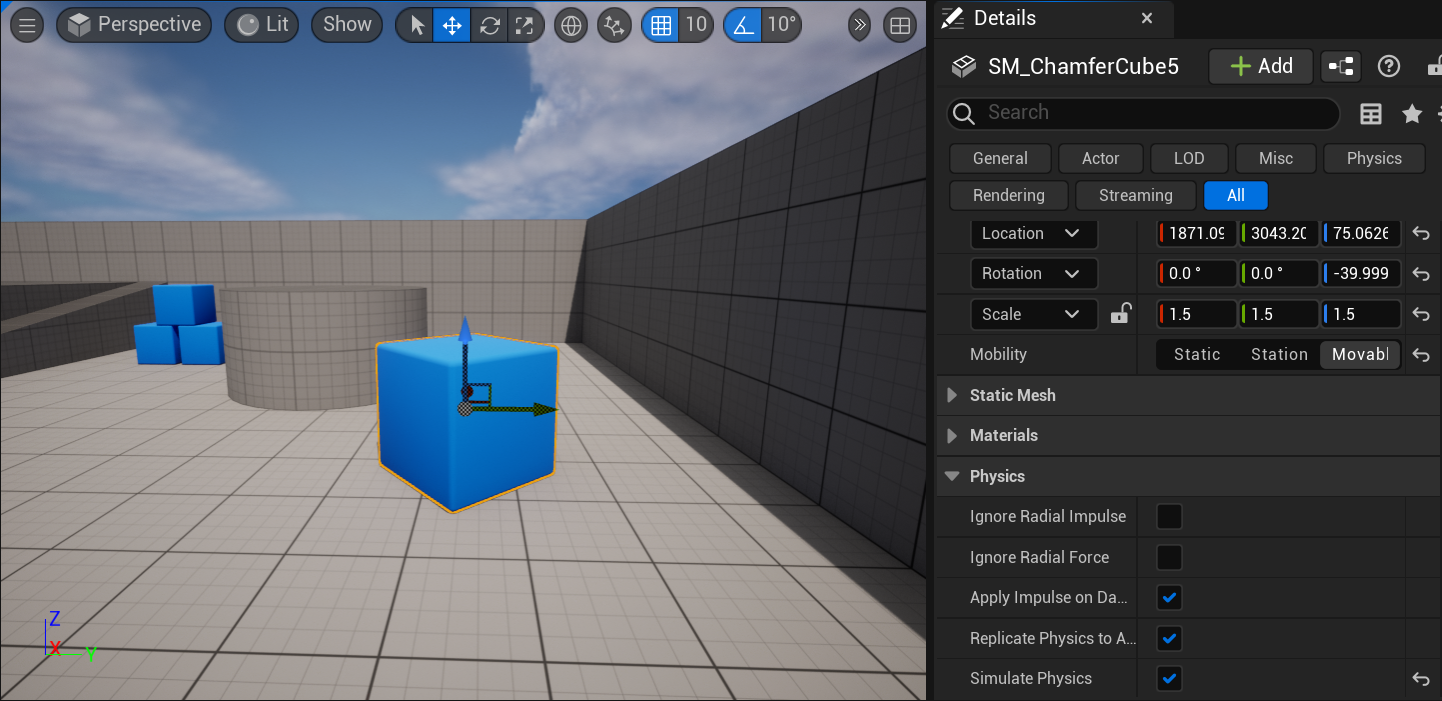
\includegraphics[width=16cm]{Images/Chap3/unreal.png}
    \caption{GUI screenshot of Unreal}
    \label{req:unreal}
\end{figure}

An appropriate graphical user interface is helpful for users to understand the functions the software product provides to them. Besides, the programmer can also complete the testing and debugging job through a well-designed GUI. Then we have to figure out what should a good interface looks like. The design of a successful commercial game engine inspires this question. As is shown in the screenshot of Unreal Engine (figure \ref{req:unreal}), the attributes of an object are illustrated on the GUI. In addition, the content of the visualisation can be changed through buttons and checkboxes. For this project, as discussed in \ref{req:visual}, the GUI is supposed to render a single model and its SDF in the same scene while the camera can move. Therefore, the requirement of an SDF generator GUI should contain the attributes info of the camera and several controls like checkboxes or buttons to change the visual contents of the object.

\subsection{Algorithm}
\label{req:algo}

The generation algorithm itself has been discussed in detail in the section \ref{br:algorithm1} and \ref{br:algorithm2} of Chapter \ref{chapter2}. The algorithm requirement should meet the choice mentioned in \ref{br:cAlgo}. Hence, two algorithms should be constructed for signed distance field computation, ray-tracing \cite{AkenineMller2005FastMS} and KD-tree. 

\subsection{Evaluation}
\label{req:eva}

As for evaluation, accuracy and efficiency should be considered. The result of the calculation should be saved as a text file to validate simply, while the efficiency can be evaluated through the time cost. 

\subsection{Others}

Other requirements like the multi-threading optimization should be applied to the computation process, and the project source code should be able to be compiled and running, as discussed in Chapter \ref{chapter2}. Those requirements will be considered in the system design.

\section{System Design}

\subsection{Overview}

According to the system requirement, this project will be divided into three main parts: GUI, algorithm and visualisation. In the GUI part, the Dear ImGui library will be used to implement a GUI class. In the algorithm part, three data structures of KD-Tree will be implemented as a class and used by the SDF calculation class. In the visualisation part, shaders, models, camera, and OpenGL render application is necessary for this project. Therefore, four classes will be implemented for each one. The software architecture of this project is shown in figure \ref{ds:archi}.

\begin{figure}[htbp]
    \centering
    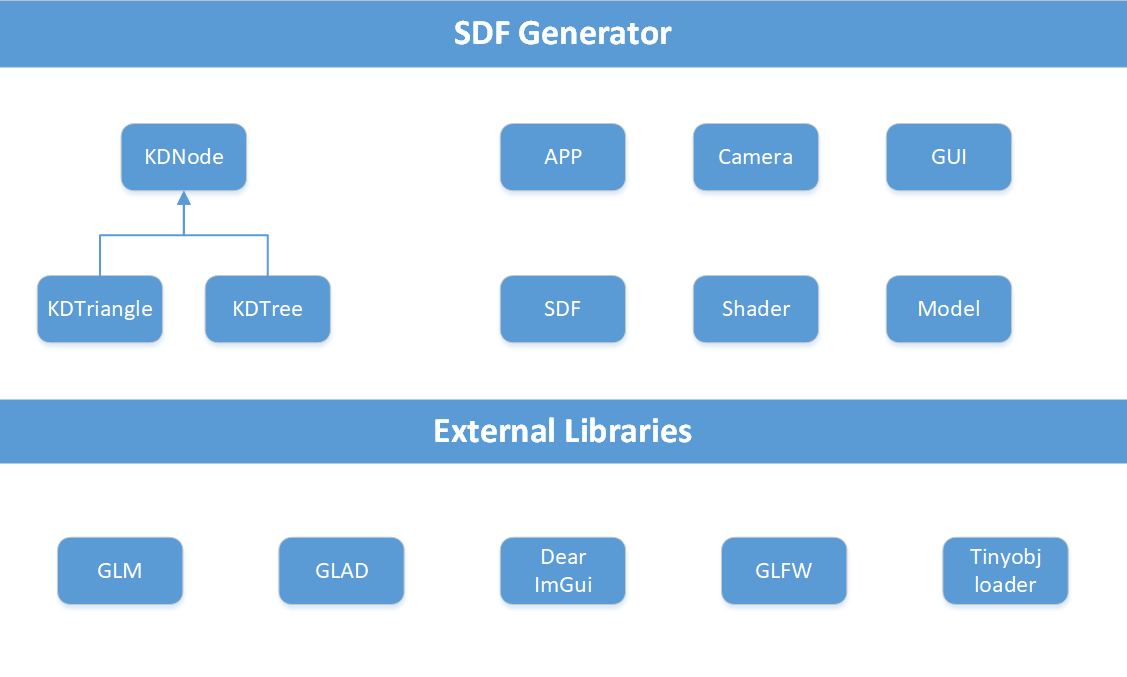
\includegraphics[width=16cm]{Images/Chap3/Architecture.png}
    \caption{The software architecture}
    \label{ds:archi}
\end{figure}

The detailed design of GUI, SDF algorithm and visualisation will be discussed in the following part of this chapter.

\subsection{Graphical User Interface}

As mentioned in \ref{br:ctpl}, the user interface will be implemented through Dear ImGui. ImGui is easily used to create a moveable control panel in front of the rendering widget. Therefore, the control options for rendering, the attributes of the camera and the debug info like generation time will be set on a moveable panel. The status of rendering control options can be changed through checkboxes. The GUI design is shown below in figure \ref{ds:gui}. 

\begin{figure}[htbp]
    \centering
    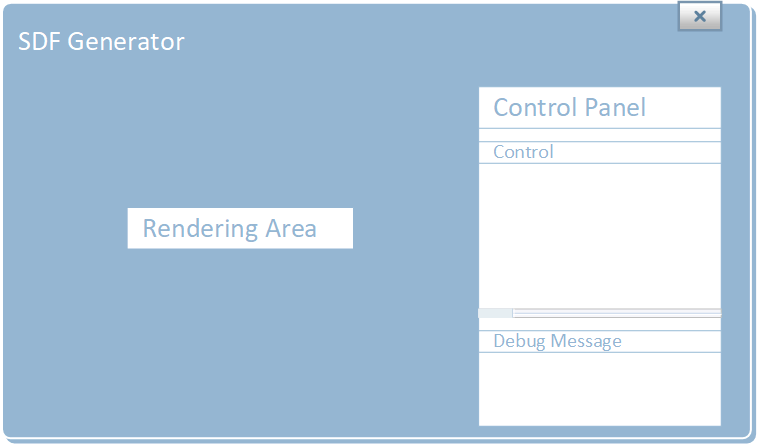
\includegraphics[width=15cm]{Images/Chap3/GUIdesign.png}
    \label{ds:gui}
    \caption{The application GUI design}
\end{figure}

\subsection{Algorithm}

There are three main algorithms to complete the signed distance field computation: the KD-tree structure, ray intersection and field generation.

\subsubsection{KD-Tree}
The tree should be built initially to use the KD-tree as the acceleration structure. As the project aims to generate a signed distance field for triangular meshes, the primitives of the tree should be triangles, which will be set as the tree node's data structure. Therefore, the nodes are constituted by the essential elements of triangles, i.e. vertices and edges. Besides, the bounding boxes and normal information will be stored in the nodes. To accelerate the process of ray intersection judgement, the function will be contained in the node structure.

\hspace*{\fill}

The structure of the KD-tree is shown in figure \ref{ds:kd}. The pseudocode of building the KD-tree algorithm is shown as Algorithm \ref{ds:kdbuild}.

\begin{figure}[htbp]
    \centering
    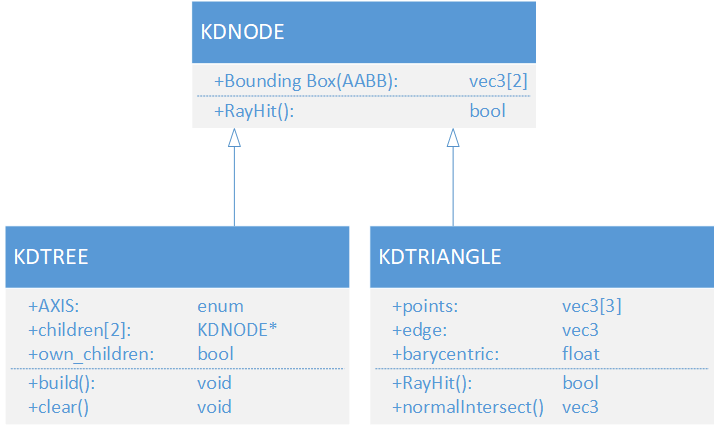
\includegraphics[width=15.5cm]{Images/Chap4/kdtree.png}
    \caption{The structure of KD-tree}
    \label{ds:kd}
\end{figure}

\subsubsection{Ray Instersection}

To apply the ray intersection algorithm, a number of sample rays must be generated equally. A sample voxel can be recognised as a sphere and split according to a fixed step. In Ahn's solution \cite{glsphere}, the sphere is divided into a number of stacks and sectors, shown as figure \ref{br:sphere}.

\begin{figure}[htbp]
    \centering
    \subfigure
    {
        \begin{minipage}[b]{.45\linewidth}
            \centering
            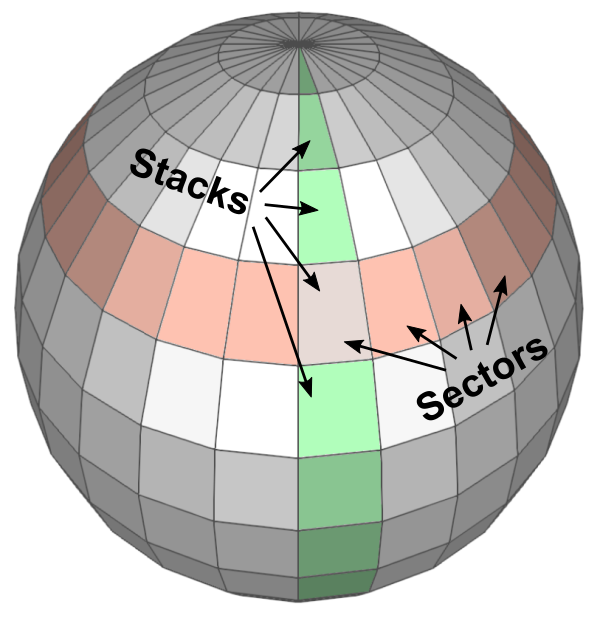
\includegraphics[width=6.5cm]{Images/Chap2/gl_sphere02.png}
        \end{minipage}
    }
    \subfigure
    {
         \begin{minipage}[b]{.45\linewidth}
            \centering
            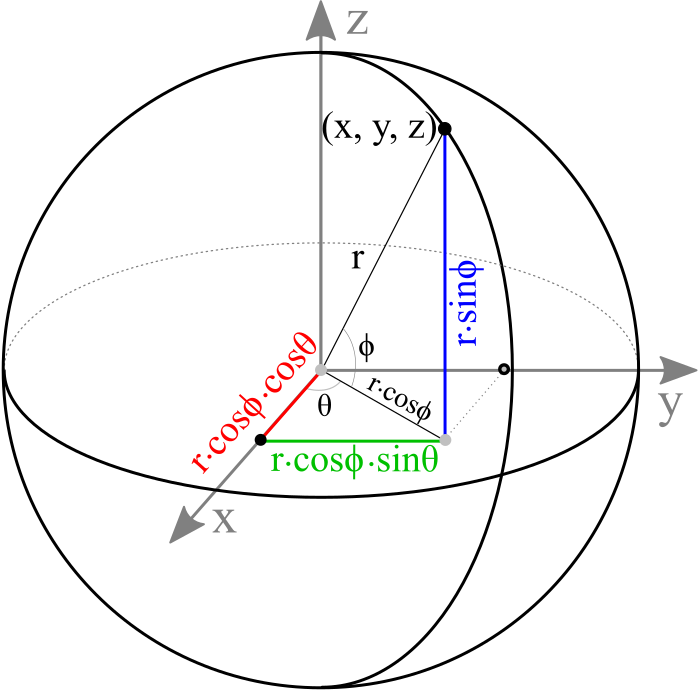
\includegraphics[width=6.5cm]{Images/Chap2/gl_sphere01.png}
        \end{minipage}
    }
    \caption{Calculate the coordinate of arbitrary point on sphere}
    \label{br:sphere}
\end{figure}

\clearpage

Then the coordinate of an arbitrary point p(x,y,z) can be computed as equation \ref{br:spherecoord}:

\begin{equation}
\label{br:spherecoord}
    \begin{aligned}
    x & = \left ( r\cdot \cos \phi  \right ) \cdot \cos \theta \\
    y & = \left ( r\cdot \cos \phi  \right ) \cdot \sin \theta \\
    z & = r\cdot \sin \phi 
    \end{aligned}
\end{equation}

Where the sector angle $ \theta $ and stack angle $ \phi $ can be calculated by equation \ref{br:sphereangle}:

\begin{equation}
\label{br:sphereangle}
   \begin{aligned}
    \theta & = 2\pi \cdot \frac{sectorStep}{sectorCount}  \\
    \phi & = \frac{\pi }{2} - \pi \cdot \frac{stackStep}{stackCount} 
    \end{aligned}
\end{equation}

\hspace*{\fill}

After generating the rays, the intersection algorithm needs to be used for distance computation. The algorithm of Tomas Akenine-M{\"o}ller and Ben Trumbore \cite{AkenineMller2005FastMS} represent a point on triangle as $ T(u, v)$, while $ (u, v) $ are the barycentric coordinates and satisfy $ u \geq 0, v \geq 0 $. Then $ T $ can be represent as \ref{br:pointT}:

\begin{equation}
    T(u, v)=(1-u-v) V_{0}+u V_{1}+v V_{2}
    \label{br:pointT}
\end{equation}

$ V_{0}, V_{1}$ and $ V_{2} $ are the vertices of triangle.

\hspace*{\fill}

We use $ R(t) $ to denote a ray of length t, then the formula for $ R(t) $ is as \ref{br:ray}:

\begin{equation}
    R(t)= O + t D
    \label{br:ray}
\end{equation}

$ O $ is the origin while $ D $ is the unit vector of direction.
Therefore, we can calculate the intersection problem by simply solving the equation \ref{br:intersection}:

\begin{equation}
    O+t D=(1-u-v) V_{0}+u V_{1}+v V_{2}
    \label{br:intersection}
\end{equation}

Which can be reordered as the linear system of equation\ref{br:interreoder}:
\begin{equation}
    \left[\begin{array}{lll}
        -D, & V_{1}-V_{0}, & V_{2}-V_{0}
        \end{array}\right]\left[\begin{array}{l}
        t \\
        u \\
        v
        \end{array}\right]=O-V_{0}
    \label{br:interreoder}
\end{equation}

let $ M=\left[-D, V_{1}-V_{0}, V_{2}-V_{0}\right] $, the ray and triangle can be transformed as \ref{br:trans}:
\begin{figure}[htbp]
    \centering
    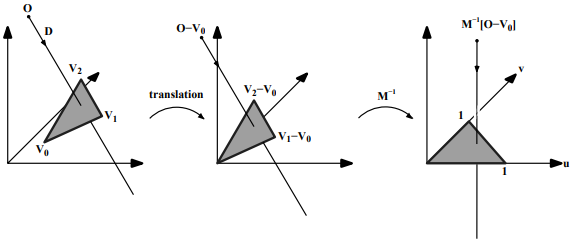
\includegraphics[width=15cm]{Images/Chap2/intersection.png}
    \caption{Translation and change of base of the ray origin}
    \label{br:trans}
\end{figure}

let $ E_{1}=V_{1}-V_{0}, E_{2}=V_{2}-V_{0} $ and $ T=O-V_{0} $, use the Cramer's rule, the equation \ref{br:interreoder} is able to be rearranged as \ref{br:reorder1}:

\begin{equation}
    \begin{bmatrix}t
        \\u
        \\v
       \end{bmatrix}=\frac{1}{\left|-D,E_{1},E_{2}\right|}
       \begin{bmatrix}\left|T,E_{1},E_{2}\right| 
        \\\left|-D,T,E_{2}\right|
        \\\left|-D,E_{1},T\right|
       \end{bmatrix}
    \label{br:reorder1}
\end{equation}

\hspace*{\fill}

Applying $ |A, B, C|=-(A \times C) \cdot B=-(C \times B) \cdot A $ to \ref{br:reorder1}, we finally get equation \ref{br:interFinal}:

\begin{equation}
    \begin{bmatrix}t
        \\u
        \\v
       \end{bmatrix}
       =\frac{1}{\left (D\times E_{2}\right)\cdot E_{1}}
       \begin{bmatrix}\left( T\times E_{1}\right)\cdot E_{2} 
        \\\left (  D\times E_{2}\right )\cdot T 
        \\\left (  T\times E_{1}\right )\cdot D
       \end{bmatrix}
       =\frac{1}{P\cdot E_{1}} \begin{bmatrix}Q\cdot E_{2} 
        \\P\cdot T 
        \\Q\cdot D
       \end{bmatrix}
    \label{br:interFinal}
\end{equation}

where $ P=\left(D \times E_{2}\right) $ and $ Q=\left(T \times E_{1}\right) $.

Finally, the distance t can be calculated as \ref{br:distance}:

\begin{equation}
    t=\frac{Q\cdot E_{2}}{P\cdot E_{1}}
    \label{br:distance}
\end{equation}

There are two branches of the ray-intersection problem. The first one is to determine whether a ray intersects with the bounding box; id Software provides a solution in DOOM3 \cite{raybound}. If the ray intersects with the bounding box, then the application will make a further determination, which is the second branch: intersect with the triangle. This algorithm will be used in the second branch to compute the distance function.

\subsubsection{Signed Distance Field Generation}

Finally, the whole distance field can be generated with the values of signed distance functions. The method of ray intersection judgement should be implemented through KD-tree acceleration and invoked by the generation algorithm.

\hspace*{\fill}

The data members of the SDF class should contain the file path, bounding box, resolutions, distance values, and sample voxels that should be stored into vectors. Besides, a generating function is necessary, and the computed values should be able to output and read in again.

\hspace*{\fill}

Figure \ref{ds:sdfclass} provide the structure of SDF class.

\begin{figure}[htbp]
    \centering
    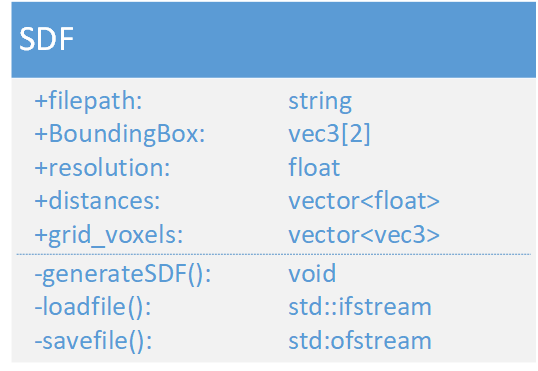
\includegraphics[width=10cm]{Images/Chap3/SDFclass.png}
    \caption{The structure of SDF class}
    \label{ds:sdfclass}
\end{figure}

\subsection{Visualisation}
\label{ds:visual}

The design of the visualisation module should contain resource loading (including shaders and models), a render scene, a scene camera and a render window.

\subsubsection{Resources Loading}
\label{ds:resource}

\paragraph{Shader}

The shader class should be about to load different types of shader files. Several enumerations can distinguish the shader type. After setting the type of shader, we can invoke the gl functions like glCompileShader() to compile shaders. Finally, the shader will be created successfully. 

\hspace*{\fill}

The structure of the shader class and its members are shown in figure \ref{ds:shaderclass}.

\begin{figure}[htbp]
    \centering
    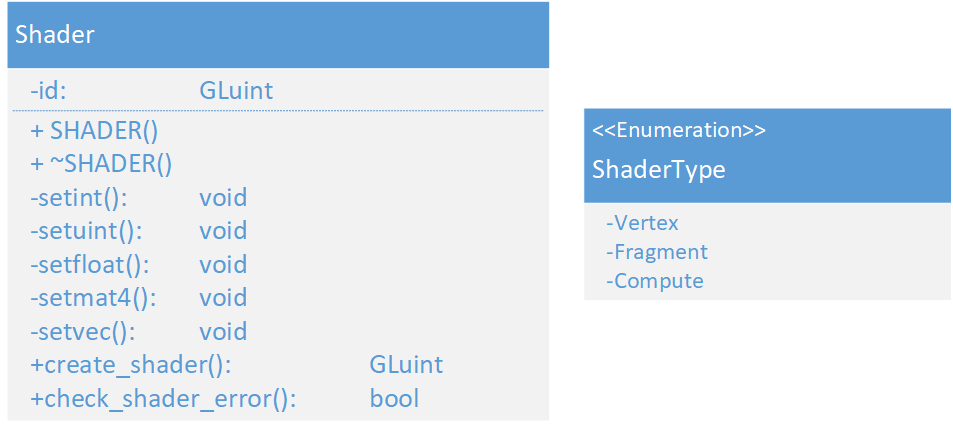
\includegraphics[width=16cm]{Images/Chap4/Shader.png}
    \caption{The structure of Shader class}
    \label{ds:shaderclass}
\end{figure}

\paragraph{Model}

The model load class used the tiniobjloader library. Considering about the requirements for computation, the information of vertices and normals will be read from the file. Then the vertices need to be reordered to the primitives, in this project, triangles. Then VAO and VBO should be created and allocated. Finally, the KD-tree should be built for the model, and the sample ray should test the intersection with the model. Therefore, both functions need to be implemented in the class.

\hspace*{\fill}

The structure of model class is shown in figure \ref{ds:modelclass}.

\begin{figure}[htbp]
    \centering
    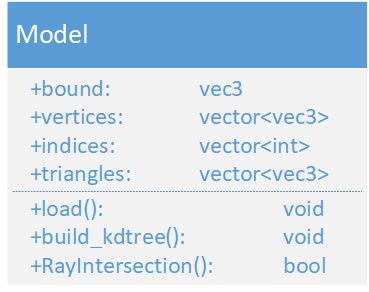
\includegraphics[width=8.5cm]{Images/Chap4/Model.png}
    \caption{The structure of Model class}
    \label{ds:modelclass}
\end{figure}

\subsubsection{Scene}

As for the scene, a grid-structured plane which can be extended infinitely is enough; the main coordinate axis will be highlighted. This plane can be implemented through a shader and can be directly reused by other applications or graphic APIs like Vulkan. Marie \cite{scene} provide the methods to create such a scene in the following order. First, create a basic grid plane vertex and fragment shader. Second, set the plane coordinates as infinity. Then draw the floor plane(i.e. y=0) and make the axis and grids on the floor. Finally, use the fragment shader to add a fade-out effect when the grid is far away.

\subsubsection{Camera}
\label{ds:camera}

The camera should be able to control by the mouse. The GLFW window will collect the user input; therefore, the camera class need to provide transformation functions like translation, rotation and zoom. Besides, the camera status should be updated by time step, and independent of the frame rate, the timer can be used for implementing the update method.

\clearpage

Figure \ref{ds:cameraclass} provides the structure of Camera class.

\begin{figure}[htbp]
    \centering
    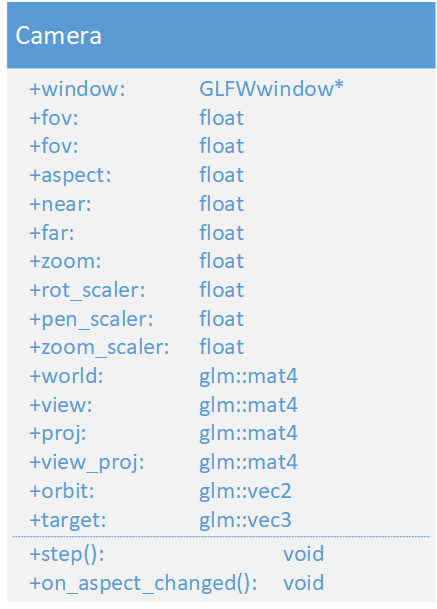
\includegraphics[width=10cm]{Images/Chap4/Camera.png}
    \caption{The structure of Camera class}
    \label{ds:cameraclass}
\end{figure}

\subsubsection{Rendering Process}
\label{ds:rendering}

The rendering process is divided into three main stages: initialize, terminate and rendering loop.

\paragraph{Initialize}

This stage contains the primary setting of an OpenGL application. A function for creating a GLFW window will be defined; other operations are contained in this function, like setting up a version and receiving the user input, which will be used to manipulate the camera. Besides, this function is also necessary for testing if the development environment has been set correctly. Then the rendering resources need to be read in, including models and shaders. If the last compute result of the signed distance field exists, it will also be loaded. If not, then the computation function will be running. Before entering the rendering loop, the parameters of the GUI will be set, and the GUI components will be bound to the same GLFW window.

\paragraph{Terminate}

The functions that tell the libraries to terminate and release the resources like glfwTerminate() have been contained in their codes, which only needs to be invoked by the terminate function.

\paragraph{Rendering}

In the rendering loop, three tasks need to be completed. First, the status of the timer needs to be stored and updated to ensure the camera transformation's stability. Then, the application will get framebuffer status and update continuously. For example, if the window has been resized, the viewport should be updated so that the pixels will be rendered properly; the swapbuffer technique \cite{Framebuffer} is applied in this process to prevent tearing or flickering issues. In addition, the GUI panel will be configured, and the contents like checkboxes and textboxes will be created and updated. Finally, the rendering function will bind different shaders when changing the modes of rendering.
\chapter{Software Implementation}
\label{chap4}

The details of implementation will be described in this chapter. The modules will be explained in the chronological order in which they were implemented.

\section{Project Building}

For arbitrary Graphics API programming, setting up the development environment is complex and time-consuming and error-prone. As discussed in \ref{premake} and \ref{premake2} the Visual Studio solution will be generated through Premake5. Premake5 only contains an execute program; the configuration needs to be written to Lua scripts. The syntax of premake scripts is fixed; it should contain the basic configurations of the project, including languages, names, platforms, source code formats and others. Premake has many valuable tokens for setting the relative directories for input and output, the different settings for platforms are distinguished through the filters. Besides, in this project, many external libraries (e.g. GLFW, GLM, ImGui) need to be contained and compiled with the source file, premake can be used to set the libraries as StaticLib projects and linked to the main project, which will keep the source code of main project independent with the libraries. 

\hspace*{\fill}

After editing the scripts, the solution can be generated by Premake correctly as shown in figure \ref{impl:premake} and \ref{impl:solution}.

\begin{figure}[htbp]
    \centering
    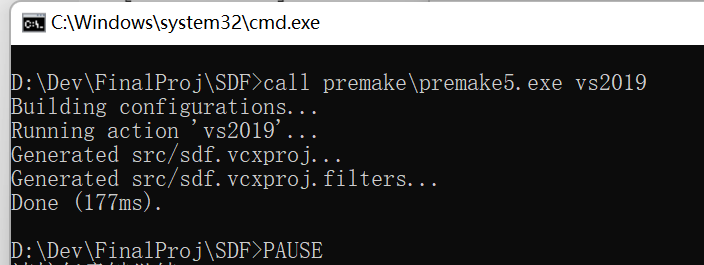
\includegraphics[width=13cm]{Images/Chap4/project.png}
    \caption{Generate Project Solution by Premake}
    \label{impl:premake}
\end{figure}

\clearpage

\begin{figure}[htbp]
    \centering
    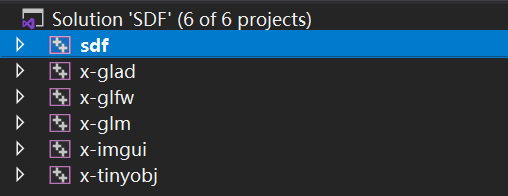
\includegraphics[width=12cm]{Images/Chap4/solution.png}
    \caption{The VS2019 Solution of this project}
    \label{impl:solution}
\end{figure}

The script code for whole solution and external libraries can be seen in Appendix \ref{ap:premake}.

\section{Basic Visualization Application}

In the first stage, a basic visualization application must be created to test whether the development environment is running properly. The modules will be implemented according to the design of the rendering process, which has been discussed in \ref{ds:visual}.

\paragraph{Shader Class}

The Shader class must load and compile shader files according to their type, and several overloaded constructors are implemented for the vertex shader, fragment shader and other options. The class invoke several gl functions for binding and compiling.

The code of constructor and creating function are shown in Listings \ref{lst:shadercons} and \ref{lst:shadercreate}.

\begin{lstlisting}[language=C++, label={lst:shadercons}, caption = Constructor of vertex and fragment shader]
    SHADER::SHADER(const char* vertex_path, const char* fragment_path)
{
    GLuint vertex_shader = create_shader(vertex_path, ShaderType::Vertex);
    GLuint fragment_shader = create_shader(fragment_path, ShaderType::Fragment);

    id = GL( glCreateProgram());
    GL( glAttachShader(id, vertex_shader) );
    GL( glAttachShader(id, fragment_shader) );
    GL( glLinkProgram(id) );

    if (check_shader_errors(id, ShaderType::Program)) exit(1);

    GL( glDeleteShader(vertex_shader) );
    GL( glDeleteShader(fragment_shader) );
}
\end{lstlisting}

\hspace*{\fill}
\hspace*{\fill}

\begin{lstlisting}[language=C++, label={lst:shadercreate}, caption = Function of creating shader]
GLuint SHADER::create_shader(const char* path, ShaderType type) const
{
    std::stringstream shader_stream;
    shader_stream << file.rdbuf();
    file.close();
    const std::string& shader_source = shader_stream.str();
    const char* shader_source_c_str = shader_source.c_str();
    GLenum shader_type = GL_VERTEX_SHADER;
    switch (type)
    {
        case ShaderType::Fragment:
            shader_type = GL_FRAGMENT_SHADER;
            break;
        case ShaderType::Compute:
            shader_type = GL_COMPUTE_SHADER;
            break;
    }
    GLuint SHADER = GL( glCreateShader(shader_type) );
    GL( glShaderSource(SHADER, 1, &shader_source_c_str, 0) );
    GL( glCompileShader(SHADER) );
    if (check_shader_errors(SHADER, type)) 
        return GLuint(-1);
    return SHADER;
}
\end{lstlisting}

\paragraph{Camera}

The camera class is implemented as a sphere orbit camera; the camera's position will rotate on a sphere orbit outside the object, whose centre is the centre of the object. There are several parameters needed to store the transformation matrices and scales. The project directly used the data structure provided by the GLM library for storing and computing. As for the operation mode, hold the right or middle mouse button, drag to move the camera, and use the mouse wheel to zoom. 

\hspace*{\fill}

The camera matrix transformation is implemented in the step() function and updated per frame, whose implementation can be seen in Listing \ref{lst:camerastep}.

\clearpage

\begin{lstlisting}[language=C++, label={lst:camerastep}, caption = Function of matrix transformation]
    void step( float elapse, const mouse_t &mouse ) {
    const glm::vec2& mouseD = mouse.mouseD;
    const glm::vec2& wheelD = mouse.wheelD;
    glm::vec3 delta( mouseD.x , -mouseD.y, 0 );
    // right button + mouse :rotation
    if ( mouse.button_stats[2] ) {
        orbit.x = constrain360( orbit.x + delta.y * rot_scaler );
        orbit.y = constrain360( orbit.y + delta.x * rot_scaler );
    }
    zoom = glm::clamp( -wheelD.y * zoom_scaler + _zoom, 10.f, 1000.f  );
    glm::mat4  rotation = glm::mat4( glm::rotate( glm::radians( _orbit.y ), Y ) ) * glm::mat4( glm::rotate( glm::radians( _orbit.x ), X ) )  ;
    if ( mouse.button_stats[1] ) {
        target += glm::mat3(rotation) * delta * pen_scaler ;
    }
    world = glm::translate( _target ) *  rotation * glm::translate( glm::vec3(0.f,0.f, _zoom) ) ; 
    view = glm::inverse( _world);
    proj = glm::perspective( glm::radians(_fov), _aspect, _near, _far );
    view_proj = _proj * _view;
}
\end{lstlisting}

\paragraph{GLFW Window}

An application window is necessary for rendering the GUI and models. As discussed in \ref{ds:rendering}, this project uses the GLFW library to create a rendering application. In this stage, a simple shader is used to test if the window is running correctly. A GLFW window should be instantiated to achieve the target and set the compulsory attributes, then get the user input data to control the camera. The step() function is invoked in the rendering loop function; frame time and the status of the mouse are stored in an object and passed to the Camera class for matrix computation. Listing \ref{lst:glfwinit} and \ref{lst:glfwrun} shows the code of GLFW window instantiation and rendering.

\begin{lstlisting}[language=C++, label={lst:glfwinit}, caption = GLFW window instantiation]
    GLFWwindow* window = nullptr ;
    glfwWindowHint(GLFW_OPENGL_DEBUG_CONTEXT, GL_TRUE); 
    // GL 4.5 
    glfwWindowHint(GLFW_CONTEXT_VERSION_MAJOR, 4);
    glfwWindowHint(GLFW_CONTEXT_VERSION_MINOR, 5);
    glfwWindowHint(GLFW_OPENGL_PROFILE, GLFW_OPENGL_CORE_PROFILE);
    glfwWindowHint(GLFW_OPENGL_FORWARD_COMPAT, GL_TRUE);
    // Create window with graphics context
    window = glfwCreateWindow(1280, 720, "SDF", NULL, NULL);
    if (!window)   exit(1);
\end{lstlisting}

\clearpage

\begin{lstlisting}[language=C++, label={lst:glfwrun}, caption = Rendering loop implementation]
    while (!glfwWindowShouldClose(window)) {
        // Camera update
        this->mouse.wheelD = {0,0};
        this->mouse.mouseD = {0,0};
        glfwPollEvents();
        float current = glfwGetTime();
        delta = current - last;
        accum += delta;
        last = current; 
        camera.step( delta, mouse );
        // Scene render
        glfwGetFramebufferSize(window, &screen_size.x, &screen_size.y);
        if (screen_size.x!=0 && screen_size.y!=0 ) {
            glViewport(0, 0, screen_size.x, screen_size.y);
            glClear(GL_COLOR_BUFFER_BIT | GL_DEPTH_BUFFER_BIT);

            app_draw_scene( delta );
            gui_draw(clear_color);
            glfwSwapBuffers(window);
        }
    }
\end{lstlisting}

\paragraph{Scene}

The infinite grid scene will be implemented through the vertex shader and fragment shader as the method introduced by Marie \cite{scene}. The GLSL source code can be seen in the Appendix \ref{ap:scene}. The shaders are loaded to the application and compiled by the shader class to create a shader program object, then bind the object as a part of the rendering state.

\paragraph{Graphical User Interface}

The GUI is implemented through the Dear ImGui library, and the GUI panel is created by invoking the functions of the library. First, it needs to be initialized to set the window pointer for the GUI panel. Then members of the GUI will be created. For example, ImGui::CollapsingHeader() function can be used to create an independent area on the panel, and ImGui::Checkbox() can be used to create a checkbox object on the panel.

\hspace*{\fill}

Listing \ref{lst:guimpl} shows the GUI implementation code.

\begin{lstlisting}[language=C++, label={lst:guimpl}, caption = ImGui panel implementation]
    // Setup Platform/Renderer backends
    ImGui_ImplGlfw_InitForOpenGL(window, true);
    ImGui::Begin( "Panel", 0 );
    // Visibility of model
    if (ImGui::CollapsingHeader("Visibility", ImGuiTreeNodeFlags_DefaultOpen ))
    {
        static bool shows[5];
        ImGui::Checkbox("Grid", &show_grids);
        ImGui::Checkbox("Polygon", &show_polygon );
        ImGui::Checkbox("Coloured Model", &show_color );

        ImGui::Checkbox("SDF", &show_iso );
        ImGui::Checkbox("RT Approximation", &show_sdf);
    }
    // Camera Status
    if (ImGui::CollapsingHeader("Cemera", ImGuiTreeNodeFlags_DefaultOpen)) {
        ImGui::LabelText( "Orbit", "%2.0f %2.0f" , camera._orbit.x, camera._orbit.y );
        ImGui::LabelText( "Target", "%2.0f %2.0f %2.0f", camera._target.x, camera._target.y ,camera._target.z );
        ImGui::LabelText( "Zoom", "%2.0f", camera._zoom  );
    }
    ImGui::End();
    // Rendering
    ImGui::Render();
    ImGui_ImplOpenGL3_RenderDrawData(ImGui::GetDrawData());
\end{lstlisting}

Once all of the processes have been completed, a window that renders an infinity grid scene and GUI panel can be seen on the screen as figure \ref{impl:gui}.

\begin{figure}[htbp]
    \centering
    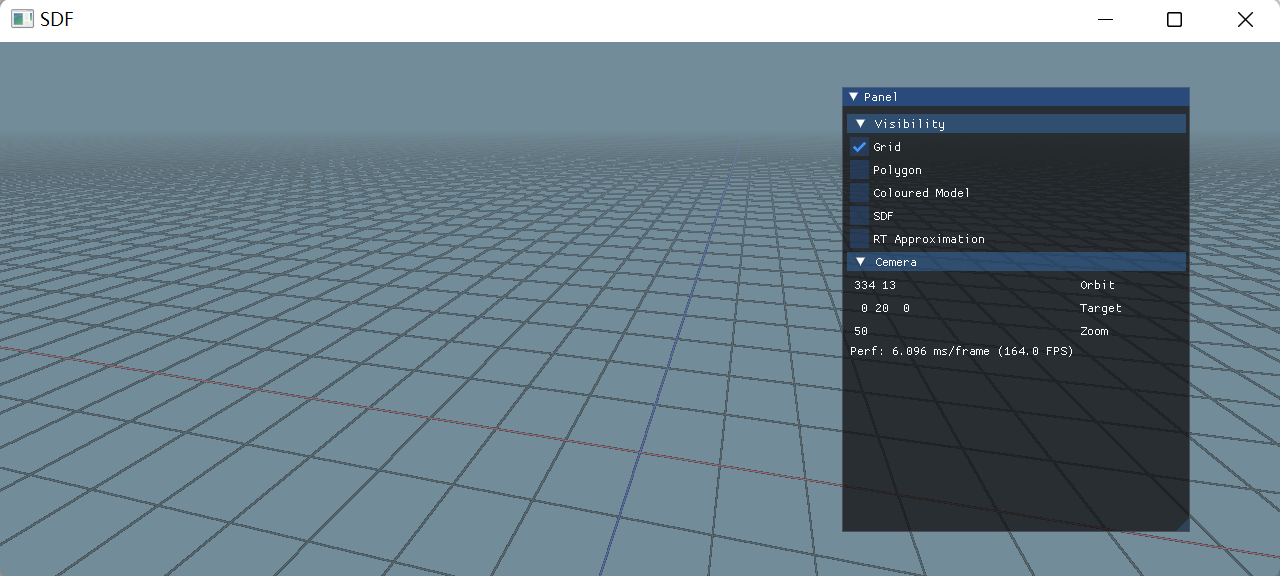
\includegraphics[width=16cm]{Images/Chap4/GUI.png}
    \caption{The basic infinity grid scene and GUI implementation}
    \label{impl:gui}
\end{figure}

\clearpage

\section{Model Rendering}

\paragraph{Model Class}

To load a triangular mesh, the tiniobjloader is used to get the vertices and face indices information. The vertices and the face indices are used to create triangle primitives for rendering and the signed distance function calculation. Several gl functions are used in the primitive creating stage.

The pseudocode of the load model is shown in Listing \ref{lst:modeload}.

\begin{lstlisting}[language=C++, label={lst:modeload}, caption = Pseudocode of model loading]
    load( obj_file ) {
    //Create empty containers
    tinyobj::attrib_t attrib;
    std::vector<tinyobj::shape_t> shapes;
    tinyobj::LoadObj(&attrib, &shapes, obj_file) // Load obj file
    // Clear the vectors
    vertices.clear();
    indices.clear();
    for (loop shape : shapes) { // Loop meshes to get vertices
        for (loop index : shape.mesh.indices) {
        vertex.pos = {
            attrib.vertices[3 * index.vertex_index + 0],
            attrib.vertices[3 * index.vertex_index + 1],
            attrib.vertices[3 * index.vertex_index + 2]    };
        vertices.push_back(vertex);     }   }   }
    triangles.resize( _indices.size()/3 );
    for ( size_t i=0;i<_triangles.size(); ++i) {
        auto i0 = _indices[i*3+0];
        auto i1 = _indices[i*3+1];
        auto i2 = _indices[i*3+2];
        triangles[i]._init( vertices[i0],vertices[i1],vertices[i2]); }
    make_primitive( vertices, indices );    }  
\end{lstlisting}

The code for making primitives are illustrated through Listing \ref{lst:modelprim}.

\begin{lstlisting}[language=C++, label={lst:modelprim}, caption = Function of creating triangular primitives]
void MODEL::make_primitive( const  vertex_t *Vdata, GLuint Vcount, 
        const uint32_t *Idata, GLuint Icount ) {
    _primitive.ibo_count = Icount;
    // Create VAO
    glGenVertexArrays(1, &_primitive.vao);
    glBindVertexArray( _primitive.vao);
    // create VBO
    glGenBuffers(1, &_primitive.vbo );
    glBindBuffer(GL_ARRAY_BUFFER, _primitive.vbo );
    // copy vertex attribs data to VBO
    GLuint vsize = sizeof(Vdata[0]) * Vcount;
    glBufferData(GL_ARRAY_BUFFER,  vsize, Vdata, GL_STATIC_DRAW);
    // Setup vertex attributes
    glVertexAttribPointer(0,3, GL_FLOAT, GL_FALSE, sizeof(Vdata[0]), 0); 
    glVertexAttribPointer(1,3, GL_FLOAT, GL_FALSE, sizeof(Vdata[0]),
        (GLvoid*) long( sizeof( Vdata[0].pos ) ));  
    glEnableVertexAttribArray(0);
    glEnableVertexAttribArray(1);        
    // Create index buffer
    glGenBuffers(1, & _primitive.ibo );
    glBindBuffer(GL_ELEMENT_ARRAY_BUFFER, _primitive.ibo );
    glBufferData(GL_ELEMENT_ARRAY_BUFFER, Icount * sizeof(Idata[0]) ,
        Idata , GL_STATIC_DRAW);  
    glBindBuffer(GL_ARRAY_BUFFER,0);
    glBindBuffer(GL_ELEMENT_ARRAY_BUFFER,0);
    glBindVertexArray(0);   }  
\end{lstlisting}

\paragraph{Rendering}

In the GUI implementation, two modes are set for model rendering, polygonal mode and coloured mode. Both can bind the same shaders, while the polygonal mode can be implemented by invoking the glPolygonMode(). The primitives of the model are set as triangles. Therefore, the draw mode should be set as GL\_TRIANGLES.

\hspace*{\fill}

Listing \ref{lst:modeldraw} shows the code of both modes.

\begin{lstlisting}[language=C++, label={lst:modeldraw}, caption = Function of creating triangular primitives]
    auto prim = &model._primitive; // Draw model primitives
    model_prog->bind(); // Bind shader
    // Setup transfrom
    model_prog->set_mat4( "MVP", glm::value_ptr( view_proj ) );
    prim->bind();
    if ( show_color ) { // Coloured draw mode
        model_prog->set_vec4( "COLOR", 0,0,0,0 );
        glDrawElements( GL_TRIANGLES , prim->ibo_count,
            GL_UNSIGNED_INT, (0) );
    }
    if ( show_polygon ) { // Polygonal draw mode
        glPolygonMode(GL_FRONT_AND_BACK, GL_LINE);
        model_prog->set_vec4( "COLOR", 1,1,1,1 );
        glDrawElements( GL_TRIANGLES , prim->ibo_count, 
            GL_UNSIGNED_INT, (0) );
        glPolygonMode(GL_FRONT_AND_BACK, GL_FILL);
    }
    prim->unbind();
    model_prog->unbind();
\end{lstlisting}

\clearpage

The result of both rendering modes can be seen in figure \ref{impl:modelrender}.


\begin{figure}[htbp]
    \centering
    \subfigure[Coloured Mode]{
        \begin{minipage}[b]{0.55\textwidth}
        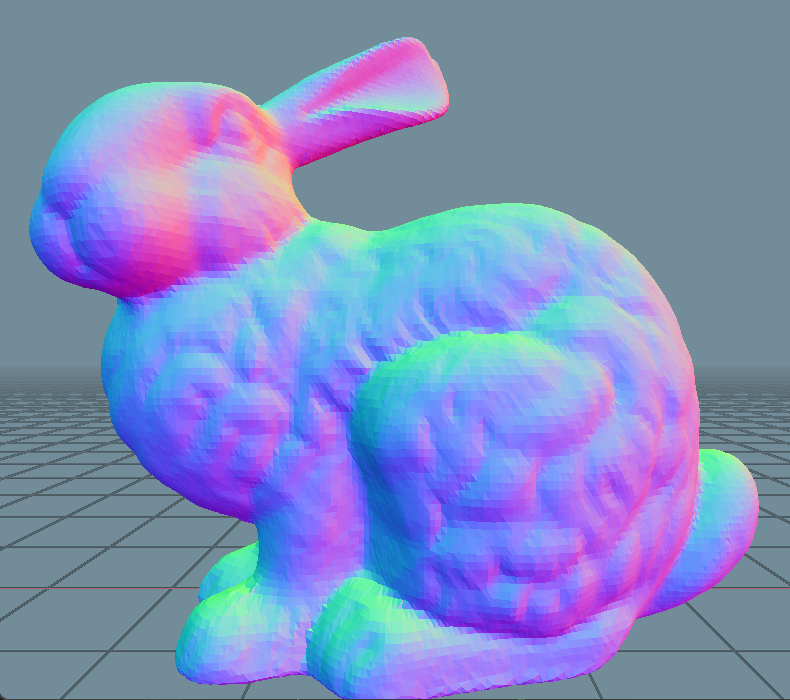
\includegraphics[width=1\textwidth]{Images/Chap4/colour.png}
        \end{minipage}
    }
    \subfigure[Polygonal Mode]{
        \begin{minipage}[b]{0.55\textwidth}
        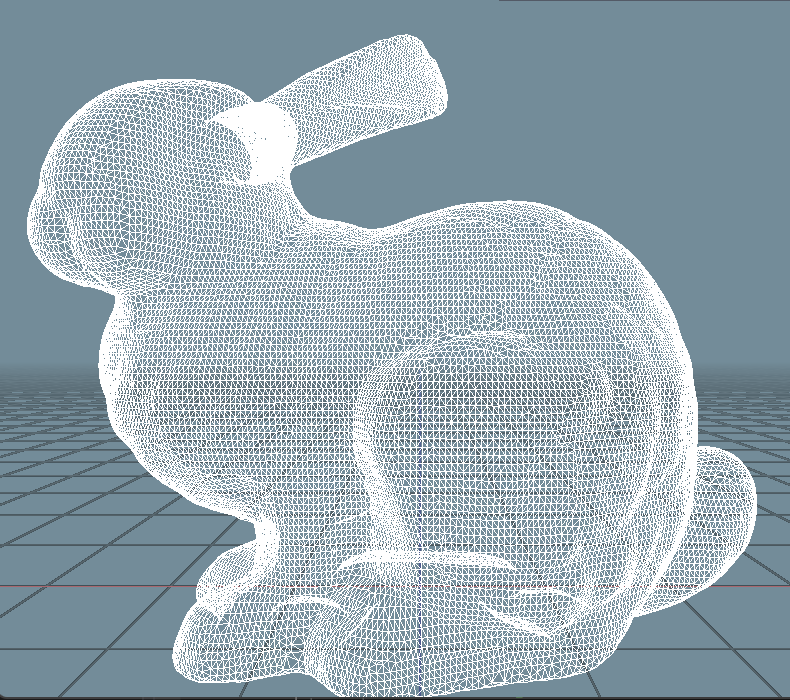
\includegraphics[width=1\textwidth]{Images/Chap4/polygon.png}
        \end{minipage}
    }
    \caption{The result of model rendering}
    \label{impl:modelrender}
\end{figure}

\section{Algorithm}

\subsection{KD-Tree}

To implement the KD-tree structure, the tree node needs to define a tree node class and then define the tree class as the derived class of the node. Since the primitives of a model are triangles, the triangle tree nodes need more data members to store their attributes like vertices and edges, while the tree class need children pointers and the split axis. Therefore, the node class is defined as an abstract class inherited by the triangle and tree class to add more variables.

\begin{breakablealgorithm}
    \caption{KD-Tree Building}
    \label{ds:kdbuild}
    \begin{algorithmic}

        \Require objects
        \State Building bounding box
        \State Set split Axis
        \Statex
        \State split bounding box
        \For{each objects i}
        \If{object[i].Bbox.center < objects.Bbox.middle}\\
                \Comment{Bbox is the bounding box of current object}
        
        \State Insert to left tree
        \Else
        \State Insert to right tree
        \EndIf
        \EndFor
        \State newBbox = left.Bbox + right.Bbox
    \end{algorithmic}
\end{breakablealgorithm}

\subsection{Ray Intersection}

There are three situations of ray-model intersection problem. If the ray start point is inside the bounding box, then the intersection status is set as true. If the ray intersects with any axis, the return value is also set as true. Otherwise, there is no intersection.

\hspace*{\fill}

The pseudocode is provided in Algorithm \ref{alg:bboxinter} below.

\begin{algorithm}[H]
    \caption{Bounding Box Intersection}
    \label{alg:bboxinter}
    \begin{algorithmic}
        \If{ray origin is inside of Bbox}
        \State return true
        \ElsIf{ray intersect with bounding box}
        \State return true
        \Else
        \State return false
        \EndIf
    \end{algorithmic}
\end{algorithm}

After completing the judgement of the intersection between ray and bounding box, the application uses the algorithm of Tomas Akenine-M{\"o}ller and Ben Trumbore \cite{AkenineMller2005FastMS} to calculate the distance function and sign function. Then the signed distance value will be stored in the intersection object for distance value comparison.

\hspace*{\fill}

The pseudocode is provided in Algorithm \ref{alg:trinter}. The definition of variables in Algorithm \ref{alg:trinter} will follow the definitions of \cite{AkenineMller2005FastMS}, which can be double reviewed in Section \ref{br:dfc}.

\begin{breakablealgorithm}
    \caption{Triangle Intersection}
    \label{alg:trinter}
    \begin{algorithmic}
        \Require EPSILON    \Comment{minimal interval from \cite{AkenineMller2005FastMS}}
        \State ray r  \Comment{denote origin as O, direction as D}
        \State triangle vertices $ V_{0}, V_{1} $ and $ V_{2}$
        \State triangle edges $ E_{1} $ and $ E_{2} $
        \State previous intersection inter\Comment{default as infinity}
        \Statex
        \State $ P = D\times E_{2} $
        \State $ determinant = E_{1} \cdot P $    \Comment{wiil be denoted as det for short}
        \State $ T = O - V_{0} $
        \Statex
        \If{det < EPSILON}
        \State return false
        \EndIf
        \Statex
        \State $ u = T \cdot P $
        \If{u < 0 or u > det}
        \State return false
        \EndIf
        \Statex
        \State $ Q = T \times E_{1} $
        \State $ v = D \cdot Q $
        \Statex
        \If{$ v < 0 $ or $ u + v > det $}
        \State return false
        \EndIf
        \Statex
        \State $  t = Q \cdot E_{2} $
        \State $  InvDet = 1{\div} det $
        \State $  t = t * InvDet $
        \If{$ t < inter.t $ and $ t > EPSILON $}
        \State update inter variable
        \State return true
        \Else \hspace{2pt} return false
        \EndIf
    \end{algorithmic}
\end{breakablealgorithm}

\subsection{Signed Distance Field Generation}

Finally, the ray intersection algorithm is applied to the field generation function. As discussed in the \ref{br:algorithm2}, each sampling voxels generate a number of rays from its centre to test and compute the distance. The first step is to loop a single voxel's ray group and get its minimal distance; the Algorithm \ref{alg:trinter} is used for single ray intersection judgement. Then test if the ray start point is inside the model or if the model has a hole to determine the sign of this voxel. Finally, record the signed distance value and repeat the process to each voxel. The ray intersection computation algorithm is implemented in the KD-tree structure for pruning.

\hspace*{\fill}

Listing \ref{lst:sampleRays} provides the code of sample rays generation.

\begin{lstlisting}[language=C++, label={lst:sampleRays}, caption = Function of generating sample rays for voxels]
    vector<vec3> sampleRays;
    sampleRays.clear();
    vec3 sum(0);
    float phiOffset = PI / phiSteps * 0.5f;
    for (int phiStep = 0; phiStep < phiSteps; phiStep++)
    {
        float phi = -PI / 2.f + (PI * phiStep) / phiSteps + phiOffset;
        for (int thetaStep = 0; thetaStep < thetaSteps; thetaStep++)
        {
            float theta = (PI * 2.f * thetaStep) / thetaSteps;
            vec3 direction(cosf(theta), sinf(theta), sinf(phi));
            sum += normalize(direction);
            sampleRays.push_back(normalize(direction));
        }
    }
\end{lstlisting}

The pseudocode of the field generation algorithm is shown in Algorithm \ref{alg:sdfgen}:

\begin{breakablealgorithm}
    \caption{SDF Generation}
    \label{alg:sdfgen}
    \begin{algorithmic}
        \Require mesh, dimensions, sampleRays
        \Statex
        \State Bbox = mesh.bbox     \Comment{The bounding box of the mesh}
        \State d = dimensions
        \State hit = 0
        \State hitBack = 0
        \Statex
        \For{each point p(x,y,z) in Bbox}
            \State minDistance = $ \infty $

            \For{each ray in sampleRays}
            \If{ray intersect with model}
                \State hit++
                \If{ray intersect with backside}
                \State hitBack++
                \EndIf
                \If{currentDistance < minDistance}
                \State minDistance = currentDistance
                \EndIf
            \EndIf
            \EndFor

            \If{Over half of rays hit backside}
            \State The ray origin inside mesh
            \State sign is negative
            \EndIf

            \If{The meshes has hole}
            \State The ray origin inside mesh
            \State sign is negative
            \EndIf
        \State Distance at p(x,y,z) = minDistance
        \EndFor
    \end{algorithmic}
\end{breakablealgorithm}

The asynchronous multi-threading strategy is also applied to reduce the generation time. The voxels are divided into many groups, and each group will run the generation function in parallel. The method is implemented by using the std::async() function. 

\hspace*{\fill}

Listing \ref{lst:async} gives the code of multi-threading acceleration. The Algorithm \ref{alg:sdfgen} is implemented in function generate\_layer().

\begin{lstlisting}[language=C++, label={lst:async}, caption = Function of generating sample rays for voxels]
    auto future = std::async(std::launch::async, [&] {
        std::vector<int> zid (dfDimensions.z);
        std::iota (std::begin(zid), std::end(zid), 0); 
        
        std::for_each(
        std::execution::par,
        zid.begin(),
        zid.end(),
        [&](auto&& zIndex)
        {
            cout << "\tProcessing layer: " << zIndex << endl;
            generate_layer(model,sampleRays, 
                zIndex, _layer_progress[zIndex] );
        });
        return 0;
    });
\end{lstlisting}

\clearpage

\section{SDF output and debug}

The result of the signed distance field is stored in a text file since it is easy to be generated and validate. Operator << is overloaded to 
output the values. The implementation can be seen in Listing \ref{lst:sdfout}

\begin{lstlisting}[language=C++, label={lst:sdfout}, caption = SDF output function]
    ofstream &operator<<(ofstream &o, const SDF &data) {
        o << data._source << endl
        << data._grids.x << " " << data._grids.y << " " << data._grids.z << endl
        << data._resolution << endl;
        for (float f : data._voxels) //distance values
        {   o << f << endl;    }
        for (auto v : data._vertices) // sample voxels
        {   o << v.x << " " << v.y << " " << v.z << endl;   }
        return o;
    }
\end{lstlisting}

Some debug information needs to be shown on the interface, including generation time, triangle number and sampling resolutions. Therefore, the GUI panel implementation should add a new capsule area.

\hspace*{\fill}

The final GUI panel implementation is shown in figure \ref{impl:guidebug}.

\begin{figure}[htbp]
    \centering
    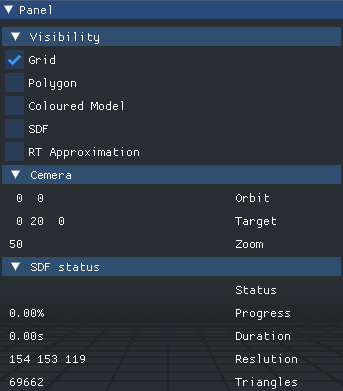
\includegraphics[width=9cm]{Images/Chap4/guidebug.png}
    \caption{GUI panel with debug info}
    \label{impl:guidebug}
\end{figure}

\clearpage

\section{SDF Visualization}
\label{impl:sdfvisual}

Finally, the result of the SDF calculation should be visualized. Two methods are implemented in this project, and the first one is using distance values to adjust the colour value; the volume of colour is changed according to the distance. The result is shown in figure \ref{impl:sdfiso},  the volume of green is set as the highest on the boundary of the model while the colour of inside voxels is visualized as red. The other one used ray tracing to approximate the model shape, which is shown in figure \ref{impl:sdfrt}.

\begin{figure}[htbp]
    \centering
    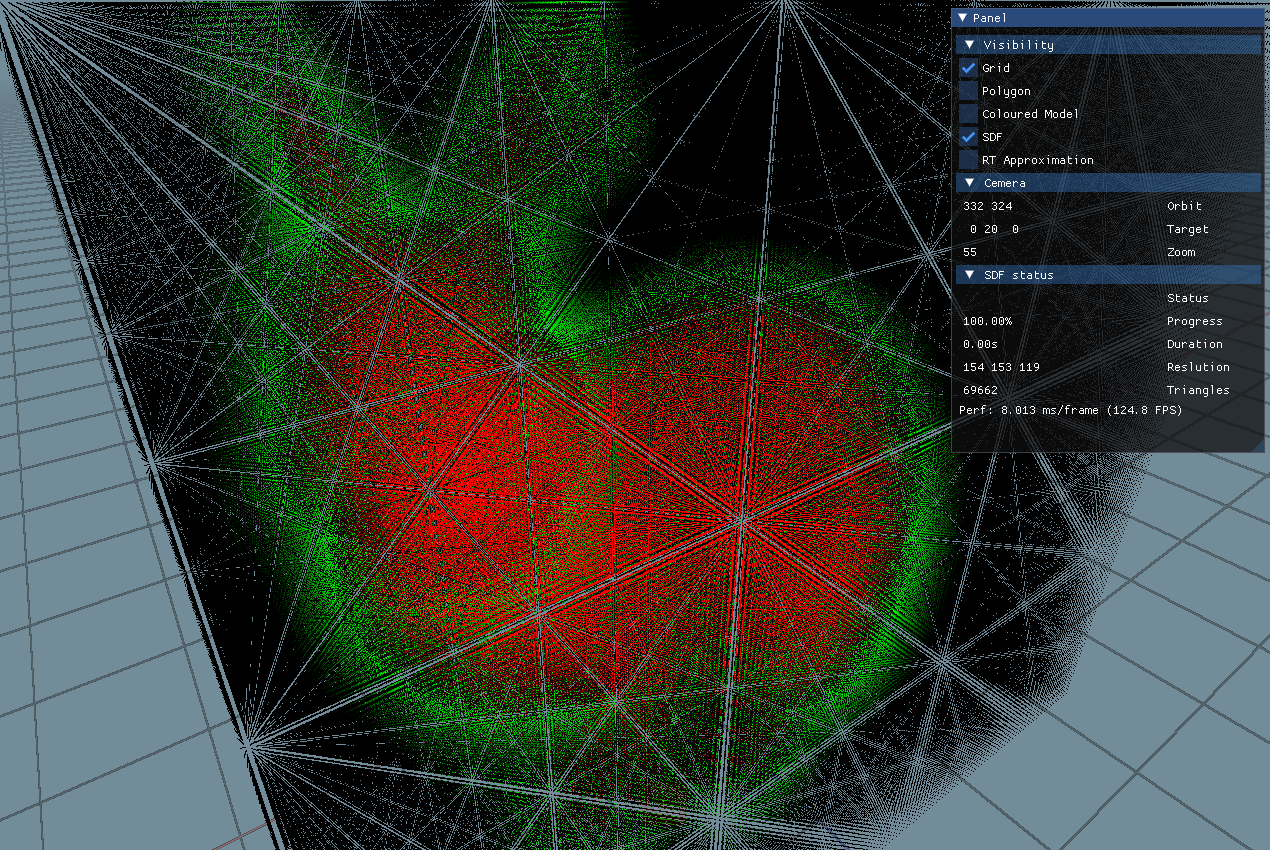
\includegraphics[width=12.6cm]{Images/Chap4/result.png}
    \caption{The colour volume mode of SDF visualization}
    \label{impl:sdfiso}
\end{figure}
\begin{figure}[htbp]
    \centering
    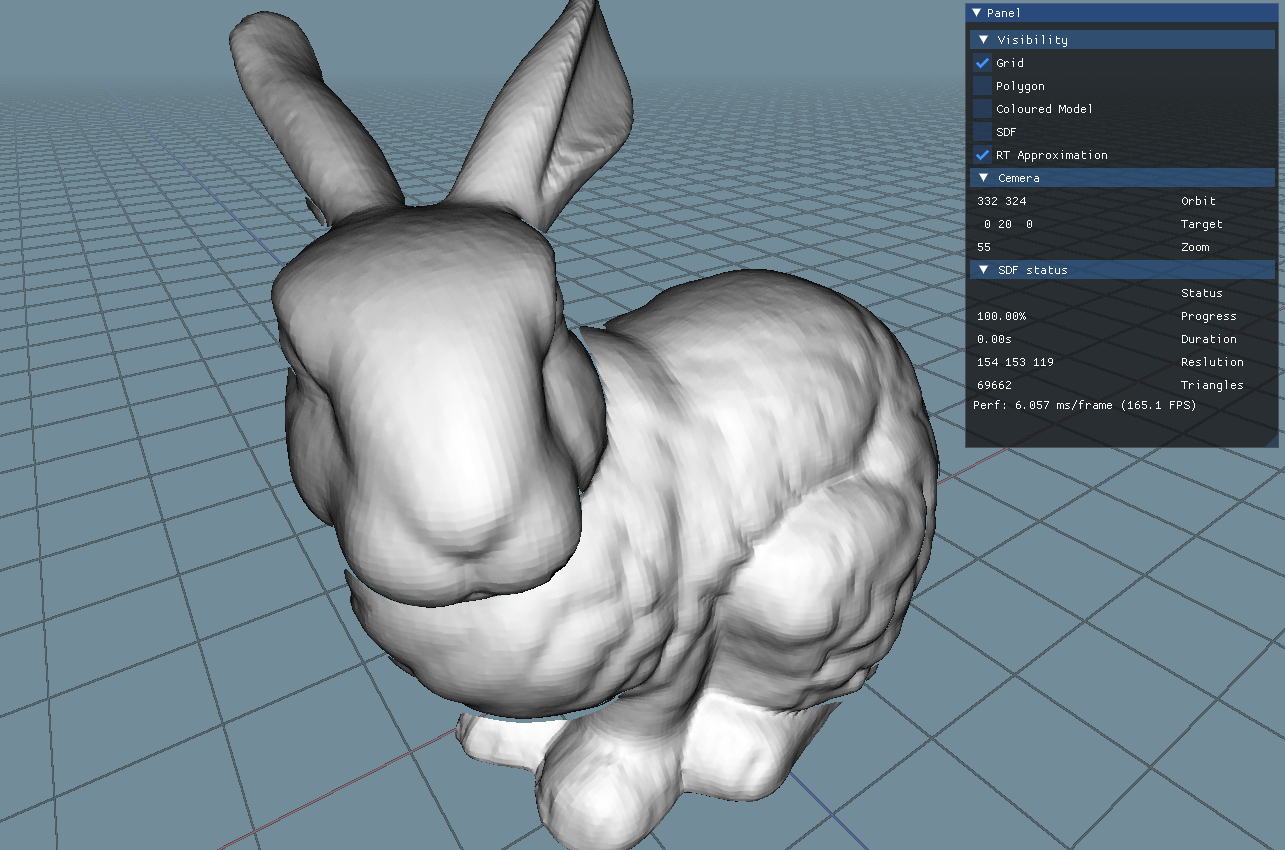
\includegraphics[width=12.6cm]{Images/Chap4/rta.png}
    \caption{The ray tracing mode of SDF visualization}
    \label{impl:sdfrt}
\end{figure}


\clearpage
\chapter{Software Testing and Evaluation}
\label{chap5}

To assess the quality of implementation, ensuring each component of this project works properly has top priority, and then the different input settings should be explored. Therefore, this chapter covers the unit test and performance evaluation to prove that the project satisfied the requirements of the initial objectives.

\section{Unit Test}

The unit test needs to verify several components: basic model rendering, GUI update and SDF.

\subsection{External Libraries}

Most of the components are implemented based on several third-party libraries. For example, the model class use the vector definition from the GLM library to store the vertices. Therefore, all libraries should ensure that they are imported correctly so that further programming and testing tasks.

\hspace*{\fill}

GLFW and GLAD testing can be verified through an executable rendering window. Once the libraries are appropriately set, the rendering pipeline is built automatically so that the GPU will render the correct image. GLM and tinyobjloader are required to be adequately included in the source code, and both can be verified through read-in a simple mesh like a cube and converting the object data to the format of GLM; if the code can be compiled and running correctly, both libraries are successfully imported. Similarly, the Dear ImGui library's import status can be verified by rendering a simple GUI component to the application window.

\hspace*{\fill}

Figures \ref{impl:gui} and \ref{impl:modelrender} have proven that the rendering pipeline, GUI library, and obj loader library have been imported properly.

\subsection{Model Rendering}

The application is supposed to process arbitrary obj files. Therefore, both simple and complex meshes are tested for this component, including the simple cube, sphere meshes and common 3D models like Spot, Stanford Bunny and Stanford Lucy. All test models can be read-in and rendered correctly through polygonal and coloured mode.

\hspace*{\fill}

The result of model rendering testing for different meshes is shown in figure \ref{ut:model}.

\begin{figure}[htbp]
    \centering
    
    \subfigure[Cube]{
    \begin{minipage}[t]{0.325\linewidth}
        \centering
        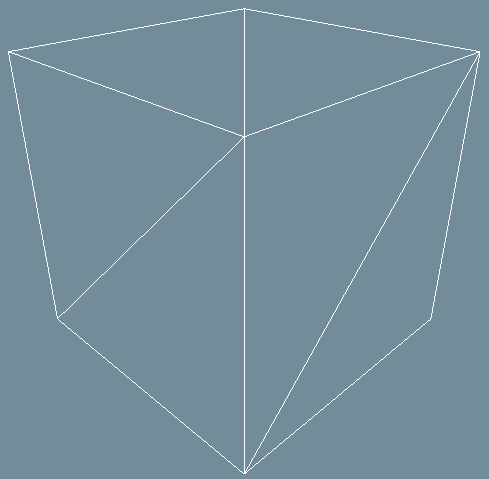
\includegraphics[width=1.5in]{Images/Chap5/cube_p.png}
        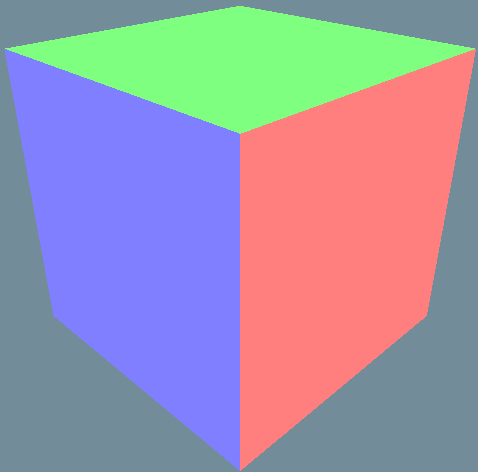
\includegraphics[width=1.5in]{Images/Chap5/cube_c.png}
    \end{minipage}%
    }%
    \subfigure[Sphere]{
    \begin{minipage}[t]{0.325\linewidth}
        \centering
        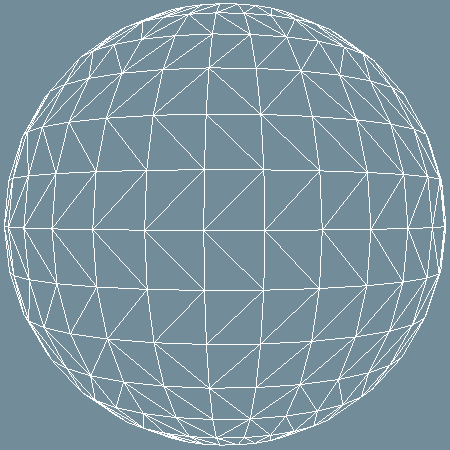
\includegraphics[width=1.5in]{Images/Chap5/sphere_p.png}
        
\includegraphics[width=1.5in]{Images/Chap5/sphere_c.png}
    \end{minipage}%
    }%
    \subfigure[Stanford Bunny]{
    \begin{minipage}[t]{0.325\linewidth}
        \centering
        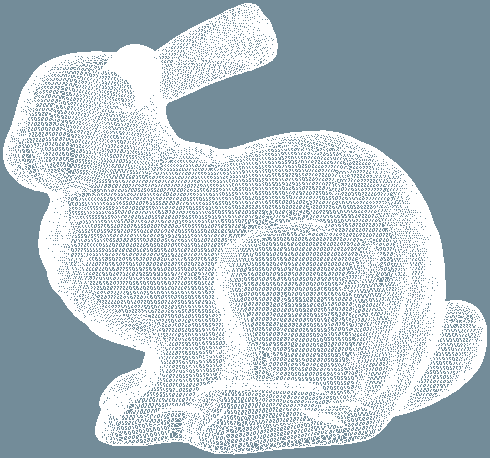
\includegraphics[width=1.5in]{Images/Chap5/bunny_p.png}
        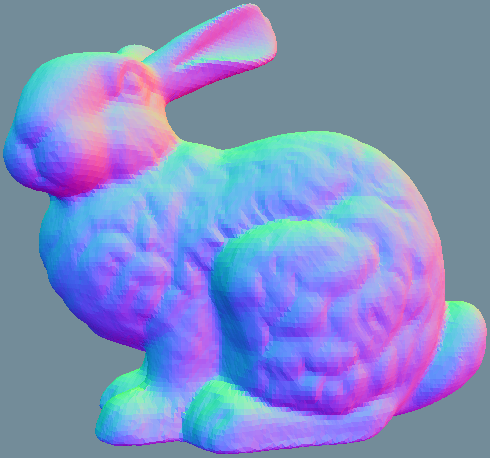
\includegraphics[width=1.5in]{Images/Chap5/bunny_c.png}
        %\caption{fig2}
    \end{minipage}
    }%
    
    \quad
    
    \subfigure[Spot]{
    \begin{minipage}[t]{0.5\linewidth}
        \centering
        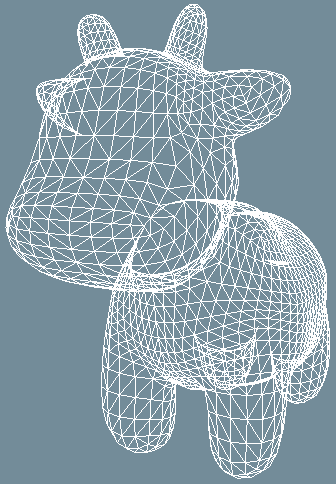
\includegraphics[width=1.5in]{Images/Chap5/spot_p.png}
        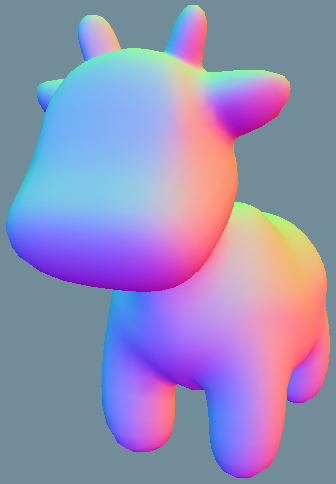
\includegraphics[width=1.5in]{Images/Chap5/spot_c.png}
        %\caption{fig2}
    \end{minipage}
    }%
    \subfigure[Stanford Lucy]{
    \begin{minipage}[t]{0.5\linewidth}
        \centering
        
\includegraphics[width=1.5in]{Images/Chap5/lucy_p.png}
        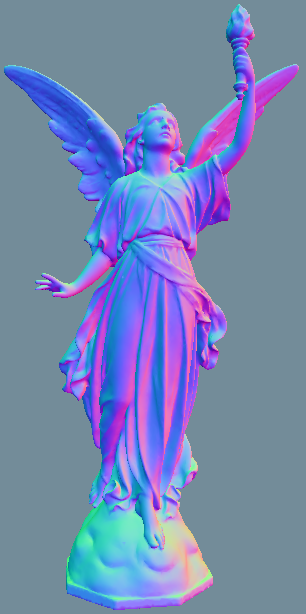
\includegraphics[width=1.5in]{Images/Chap5/lucy_c.png}
        %\caption{fig2}
    \end{minipage}
    }%
    \centering
    \caption{Rendering test for several models}
    \label{ut:model}
\end{figure}

\subsection{GUI update}

Since the computation is time-consuming, the application needs to monitor the progress of computation; the percentage of the whole model computation is shown in the debug area of the GUI panel. The GUI debug status should keep updating during the process of computing the signed distance field and provide a hint when it is finished. 

\clearpage

The GUI panel updates the computation status properly and provides the rendering hint when the computation is finished, as shown in figure \ref{ut:guiupdate}.

\begin{figure}[htbp]
    \centering
    \subfigure[Update]{
    \begin{minipage}[t]{0.495\linewidth}
        \centering
        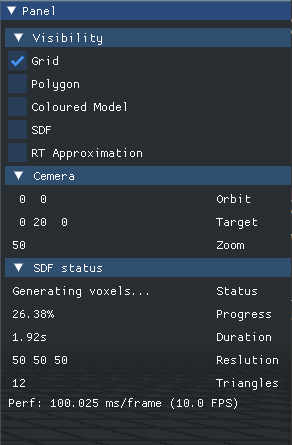
\includegraphics[width=3in]{Images/Chap5/GUIupdate.png}
    \end{minipage}%
    }%
    \subfigure[Sphere]{
    \begin{minipage}[t]{0.495\linewidth}
        \centering
        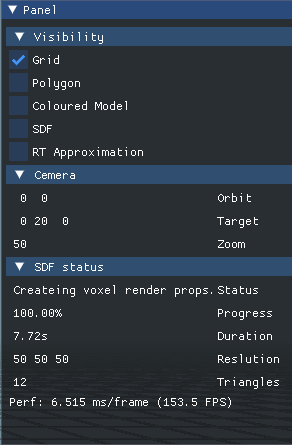
\includegraphics[width=3in]{Images/Chap5/GUIfinish.png}
    \end{minipage}%
    }%
    \caption{The Debug status update properly}
    \label{ut:guiupdate}
\end{figure}

\subsection{SDF}
\label{eva:sdf}

If the SDF has been calculated, the application reads in the generated SDF file to visualize the signed distance field. As shown in \ref{impl:sdfvisual}, the field of Stanford Bunny can be visualized properly. The result of other models can be seen in figure \ref{ut:sdfsphere}, \ref{ut:sdfspot} and \ref{ut:sdflucy}. The effect of different parameter settings on the quality of the SDF is discussed in \ref{eva:quality}.

\begin{figure}[htbp]
    \centering
    \subfigure[Colour Volume]{
    \begin{minipage}[t]{0.245\linewidth}
        \centering
        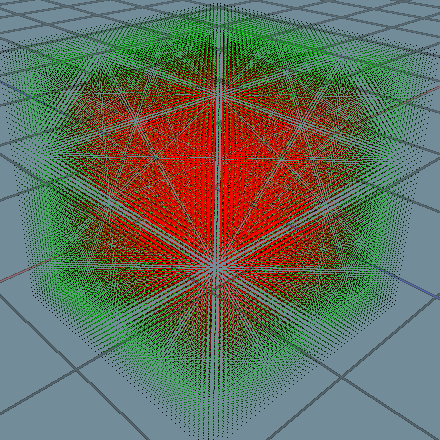
\includegraphics[width=1.3in]{Images/Chap5/cubeiso.png}
    \end{minipage}%
    }%
    \subfigure[Ray Tracing]{
    \begin{minipage}[t]{0.245\linewidth}
        \centering
        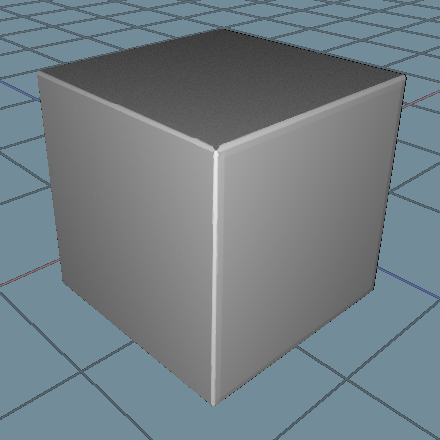
\includegraphics[width=1.3in]{Images/Chap5/cubert.png}
    \end{minipage}%
    }%
    \subfigure[Colour Volume]{
    \begin{minipage}[t]{0.245\linewidth}
        \centering
        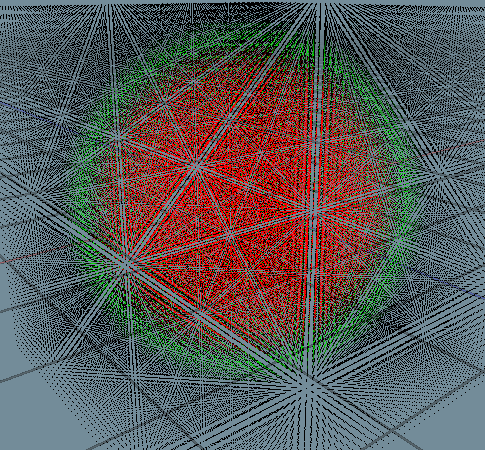
\includegraphics[width=1.4in]{Images/Chap5/sphereiso.png}
    \end{minipage}%
    }%
    \subfigure[Ray Tracing]{
    \begin{minipage}[t]{0.245\linewidth}
        \centering
        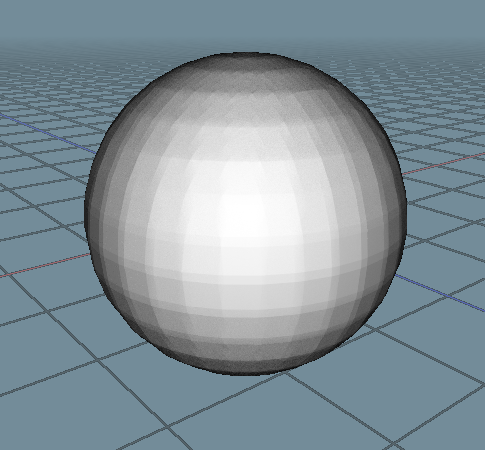
\includegraphics[width=1.4in]{Images/Chap5/spherert.png}
    \end{minipage}%
    }%
    \caption{The SDF visualization of Cube(a,b) and Sphere(c,d)}
    \label{ut:sdfsphere}
\end{figure}


\begin{figure}[htbp]
    \centering
    \subfigure[Colour Volume]{
    \begin{minipage}[t]{0.495\linewidth}
        \centering
        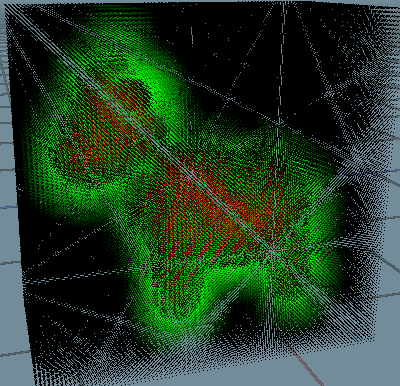
\includegraphics[width=3in]{Images/Chap5/spotiso.png}
    \end{minipage}%
    }%
    \subfigure[Ray Tracing Approximation]{
    \begin{minipage}[t]{0.495\linewidth}
        \centering
        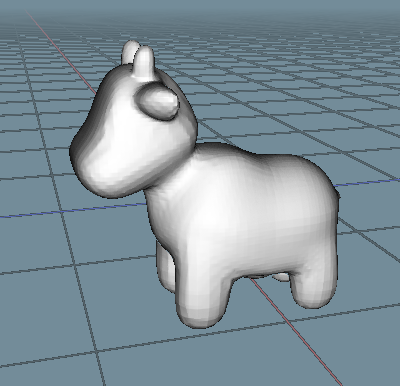
\includegraphics[width=3in]{Images/Chap5/spotrt.png}
    \end{minipage}%
    }%
    \caption{The SDF visualization of Spot}
    \label{ut:sdfspot}
\end{figure}

\begin{figure}[htbp]
    \centering
    \subfigure[Colour Volume]{
    \begin{minipage}[t]{0.495\linewidth}
        \centering
        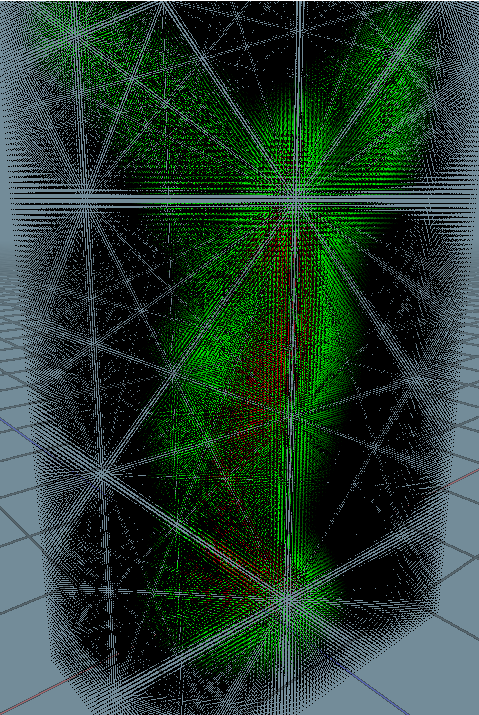
\includegraphics[width=3in]{Images/Chap5/lucyiso.png}
    \end{minipage}%
    }%
    \subfigure[Ray Tracing Approximation]{
    \begin{minipage}[t]{0.495\linewidth}
        \centering
        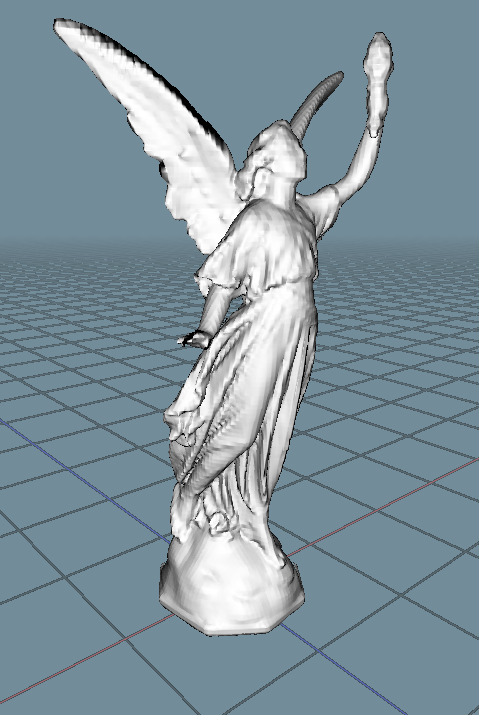
\includegraphics[width=3in]{Images/Chap5/lucyrt.png}
    \end{minipage}%
    }%
    \caption{The SDF visualization of Stanford Lucy}
    \label{ut:sdflucy}
\end{figure}

\clearpage

\section{Evaluation}

Three parameters influence the quality and generation performance of the SDF. The first one is the number of sample rays in each voxels. Another one is the resolution, which influence the number of sample voxels. The last one is triangle number of the mesh. The effect of these three parameters will be explored.

\subsection{SDF quality}
\label{eva:quality}

\subsubsection{Sample Ray Number}

The number of sample rays for each voxel affect the accuracy of distance function computation, if the ray is sparse, then the error of distance value for each sample voxel can be serious. Figure \ref{eva:rayquality} provides the SDF approximation results in different ray number settings, the resolution is set as 50*63*64.

\begin{figure}[htbp]
    \centering
    \subfigure[16 Rays]{
    \begin{minipage}[t]{0.445\linewidth}
        \centering
        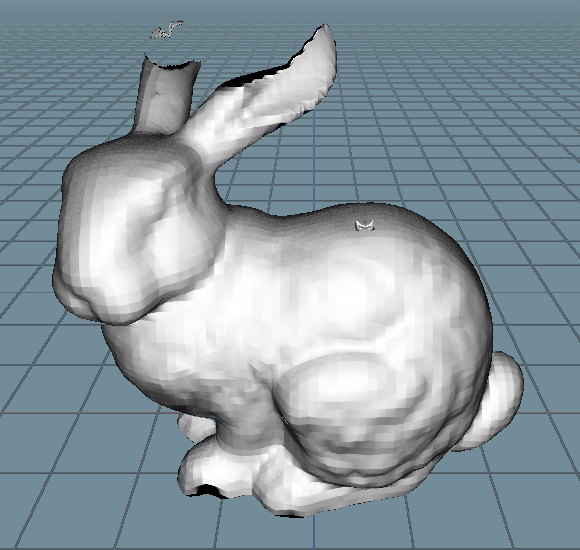
\includegraphics[width=2in]{Images/Chap5/bunny50ray16.png}
    \end{minipage}%
    }%
    \subfigure[32 Rays]{
    \begin{minipage}[t]{0.445\linewidth}
        \centering
        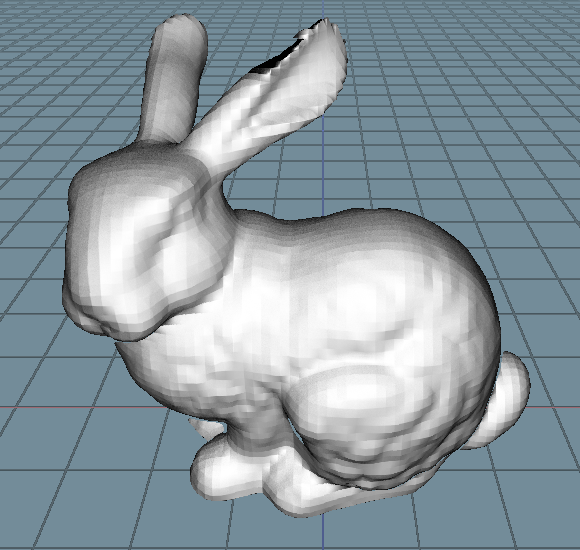
\includegraphics[width=2in]{Images/Chap5/bunny50ray32.png}
    \end{minipage}%
    }%
    \quad
    \subfigure[64 Rays]{
    \begin{minipage}[t]{0.445\linewidth}
        \centering
        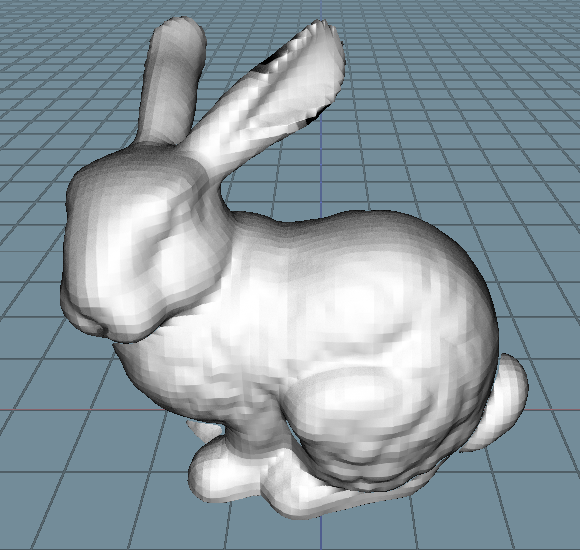
\includegraphics[width=2in]{Images/Chap5/bunny50ray64.png}
    \end{minipage}%
    }%
    \subfigure[128 Rays]{
    \begin{minipage}[t]{0.445\linewidth}
        \centering
        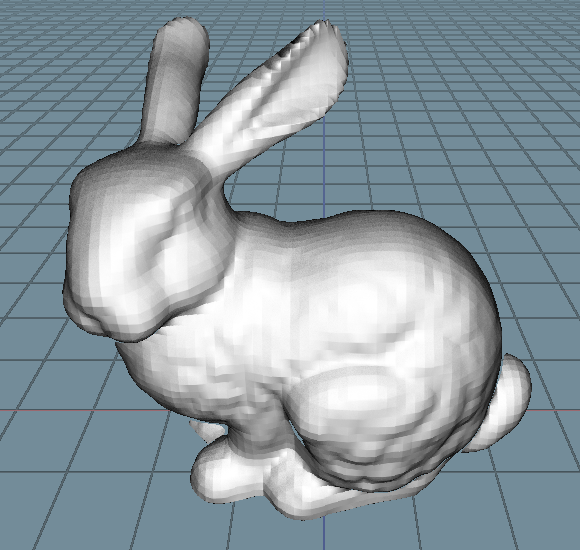
\includegraphics[width=2in]{Images/Chap5/bunny50ray128.png}
    \end{minipage}%
    }%
    \caption{The SDF approximation results for different ray number}
    \label{eva:rayquality}
\end{figure}

As can be seen in figure \ref{eva:rayquality}, when the ray number is low (a,b), there are obvious gaps in the parts of bunny'ears. As the number of rays increases, the error gradually disappears and the shape of Stanford Bunny has been nicely reproduced. Therefore, with a rational setting of ray number, the qualify of SDF generation meets the requirement.

\clearpage

\subsubsection{Resolution}

A high quality signed distance field can be generated with more sample voxels. However, using more sampled voxels can significantly increase the amount of computation and increase the generation time, especially for CPU implemented projects. In this section, the Stanford Bunny is used to explore the influence the effect of resolution on the quality of the generated SDFs since it is one of the most common 3D test model and can easily compare with other's work. The ray tracing visualisation mode is used to show the result.

\begin{figure}[htbp]
    \centering
    \subfigure[10*12*12]{
    \begin{minipage}[t]{0.325\linewidth}
        \centering
        \includegraphics[width=1.9in]{Images/Chap5/bunny10.png}
    \end{minipage}%
    }%
    \subfigure[25*31*32]{
    \begin{minipage}[t]{0.325\linewidth}
        \centering
        \includegraphics[width=1.9in]{Images/Chap5/bunny25.png}
    \end{minipage}%
    }%
    \subfigure[50*63*64]{
    \begin{minipage}[t]{0.325\linewidth}
        \centering
        \includegraphics[width=1.9in]{Images/Chap5/bunny50.png}
    \end{minipage}%
    }%
    \quad
    \subfigure[120*153*154]{
    \begin{minipage}[t]{0.475\linewidth}
        \centering
        \includegraphics[width=2.45in]{Images/Chap5/bunny120.png}
    \end{minipage}%
    }%
    \subfigure[DeepSDF \cite{park2019deepsdf}]{
    \begin{minipage}[t]{0.475\linewidth}
        \centering
        \includegraphics[width=2.15in]{Images/Chap5/bunnyDeep.png}
    \end{minipage}%
    }%
    \caption{The SDF approximation results for different resolutions and comparison with DeepSDF \cite{park2019deepsdf}}
    \label{eva:resquality}
\end{figure}

As shown in figure \ref{eva:resquality}, the shape can be roughly reproduced with a resolution of 25*31*32. The recover result of DeepSDF \cite{park2019deepsdf} is more smooth but lose a lot of details like the fur balls. Conversely, when setting the voxel number on the shortest axis as 120, the most details of the Stanford Bunny mesh can be recovered. Therefore, the quality of SDF is satisfying in this resolution.

\clearpage

\subsection{Performance}

This section will explore the influence of resolution, sample ray number and mesh triangle number on the generation performance. The evaluation has experimented on the computer of the School of Computing.

\hspace*{\fill}

The configuration of the testing computer is as follows:

\hspace*{\fill}

\begin{tabular}{ll}
    CPU & Intel 11th Gen Core i7-11700 2.5GHz\\
    RAM & 32GB DDR4 3200MHz\\
    GPU &  NVIDIA GeForce RTX 3080\\
    OS & Windows 10 Enterprise x64 20H2
\end{tabular}

\subsubsection{Sample Ray Number}

The cube with 12 triangles is used to test the influence of the sample ray number since the influence of the triangle number can be avoided in this setting. The number of sample voxels is set as 6.4k to show the change in generation time. The results can be seen in figure \ref{eva:rayper}.

\begin{figure}[htbp]
    \centering
    \includegraphics[width=14cm]{Images/Chap5/Ray.png}
    \caption{Generation time results with various ray number}
    \label{eva:rayper}
\end{figure}

As shown in figure \ref{eva:rayper}, the generation time rises linearly as the ray number increases. Therefore, the generation time is only related to the number of rays for each sample voxel when other parameters are unchanged.

\subsubsection{Resolution}

The resolution influence is tested through common 3D models: SPhere, Spot, Stanford Bunny and Stanford Lucy, while the ray number is set as 64 per voxel. The results can be seen in figure \ref{eva:resper}.

\begin{figure}[htbp]
    \centering
    \subfigure[Sphere]{
    \begin{minipage}[t]{0.485\linewidth}
        \centering
        \includegraphics[width=3in]{Images/Chap5/ResSphere.png}
    \end{minipage}%
    }%
    \subfigure[Spot]{
    \begin{minipage}[t]{0.485\linewidth}
        \centering
        \includegraphics[width=3in]{Images/Chap5/ResSpot.png}
    \end{minipage}%
    }%
    \quad
    \subfigure[Stanford Bunny]{
    \begin{minipage}[t]{0.485\linewidth}
        \centering
        \includegraphics[width=3in]{Images/Chap5/ResBunny.png}
    \end{minipage}%
    }%
    \subfigure[Stanford Lucy]{
    \begin{minipage}[t]{0.485\linewidth}
        \centering
        \includegraphics[width=3in]{Images/Chap5/ResLucy.png}
    \end{minipage}%
    }%
    \label{eva:resper}
\end{figure}

As shown in figure \ref{eva:resper}, as the voxel number increase, the SDF generation time experience a linear growth. At this point, the generation time is only positively correlated with the number of voxels. Besides, as seen from the figure, generating the SDF with around 800 thousand sample voxels can be finished within 20 seconds.

\subsubsection{Mesh Triangle Number}

The sphere meshes with different numbers of triangles are used to test the influence of mesh triangle numbers, which can avoid the influence of model shape. The sphere with 1k, 5.5k, 7.5k, 9k and 13k triangles are used, while the ray number per voxel is still set as 64. The results can be seen in figure \ref{eva:triper}.

\clearpage

\begin{figure}[htbp]
    \centering
    \includegraphics[width=14cm]{Images/Chap5/Triangle.png}
    \caption{Generation time results with various triangle number}
    \label{eva:triper}
\end{figure}

As shown in figure \ref{eva:triper}, the different triangle number affects the slope of the generation time with respect to the number of voxels. For the models with shape, generating an SDF with the same sample voxels cost more time if the mesh triangle number is larger.
\chapter{Conclusions and Future Work}

\section{Conclusions}

In this section, the objectives will be reviewed and evaluated based on the implementation, and then the existing problems will be summarised and finally, a conclusion.

\hspace*{\fill}

There are five objectives set in the planning stage. The first one is an OpenGL model visualisation application completed on June 27th, three days earlier than initially planned. The implementation of the SDF generation algorithm consumes the most time. The generation function initially used the brutal force method to ensure the data structure was built correctly; this process cost one week. Then the ray-intersection algorithm was implemented in four days and used for two days to adapt to the existing code. After that, the task became the KD-tree structure implementation, which takes the longest time to complete and test. This implementation was finished on July 20th. Then the visualisation shader of SDF was implemented four days later. Finally, the application was tested and evaluated on a personal laptop and the computer of the School of Computing and was compiled and run correctly on both. The implementation and evaluation results have been shown in Chapter \ref{chap4} and \ref{chap5}. Therefore, all of the objectives have been achieved.

\hspace*{\fill}

The main problem of this project, for now, is the performance. Although the performance is efficient for CPU implementation, using the current implementation to generate the SDF for a single complex model with satisfying quality costs of at least dozens of seconds is unacceptable for real-time rendering. In addition, the visualisation can be improved, as shown in \ref{eva:sdf}, but the result of colour volume mode is still not continuous. Besides, more visualisation modes like Ray Marching can be added. Finally, the application only supports a single model for now, which cannot meet the requirement of the modern graphic industry.

\hspace*{\fill}

In conclusion, the targets of the initial plan have been completed, and it is helpful to enhance the understanding of SDF, ray tracing and KD-tree structure. More optimisation strategies and algorithms can be added to the implementation to satisfy the requirement of modern industry and make the comparison between different solutions. Since my previous experience in computer graphics is zero, implementing this project improved my knowledge of Graphics APIs, SDF, system design, programming, evaluation and academic writing. I hope these skills will be applied to my future career.

\section{Future Work}

The main problem for the current implementation is the generation time, which can be solved by switching the implementation to GPU. The compute shader is an ideal choice. The first work for the future is implementing a GPU compute version to accelerate the generation speed. Besides, the BVH structure mentioned in \ref{br:algorithm2} is widely used in the industry. Adding BVH to the application will help compare the pros and cons of different acceleration structures. The next plan is to provide support for the complex scene. The model class should be upgraded to process the multiple meshes, which meet the realistic situation of the industrial applications. Finally, the application can be applied to more problems like sphere-tracing, soft shadow, and ray marching, and these scenarios will be gradually added to the implementation in the future.

%Adds References to the table of content
%all you bibtex enteries go in the file called refs.bib
\addcontentsline{toc}{chapter}{References}
\bibliography{refs}

%any appendices you have go in a file called appendix.
\begin{appendices}
\chapter{Premake Script}
\label{ap:premake}
%Python code highlighting
\begin{lstlisting}[caption = Premake Script for solution generation]
    workspace "SDF"
    	language "C++"
    	cppdialect "C++17"
    
    	platforms { "x64" }
    	configurations { "release", "debug" }
    
    	flags "NoPCH"
    	flags "MultiProcessorCompile"
    
    	startproject "sdf"
    
    	debugdir "%{wks.location}"
    	objdir "prebuild/%{cfg.buildcfg}-%{cfg.platform}-%{cfg.toolset}"
    	targetsuffix "-%{cfg.buildcfg}-%{cfg.platform}-%{cfg.toolset}"
    
    	filter "toolset:gcc or toolset:clang"
    		linkoptions { "-pthread" }
    		buildoptions { "-march=native", "-Wall", "-pthread" }
    	filter "toolset:msc-*"
    		defines { "_CRT_SECURE_NO_WARNINGS=1" }
    		defines { "_SCL_SECURE_NO_WARNINGS=1" }
    		buildoptions { "/utf-8" }
    		
    	filter "*"
    
    	-- default libraries
    	filter "system:linux"
    		links "dl"
    	filter "system:windows"
    	
    	filter "*"
    
    	-- default outputs
    	filter "kind:StaticLib"
    		targetdir "prebuild/lib/"
    	filter "kind:ConsoleApp"
    		targetdir "prebuild/bin/"
    		targetextension ".exe"
    		
    	filter "*"
    
    	--configurations
    	filter "debug"
    		symbols "On"
    		defines { "_DEBUG=1" }
    	filter "release"
    		optimize "On"
    		defines { "NDEBUG=1" }
    	filter "*"
    
    include "extern" 
    
    project "sdf"
    	includedirs( "src" );
    	local sources = { 
    		"src/**.cpp",
    		"src/**.hpp",
    		"src/**.hxx",
    		"src/**.h"
    	}
    
    	kind "ConsoleApp"
    	location "src"
    
    	files( sources )
    
    	links "x-glad"
    	links "x-glad"
    	links "x-glfw"
    	links "x-tinyobj"
    	links "x-imgui"
    	dependson "x-glm" 
    
    	filter "system:linux"
    		links "tbb"
\end{lstlisting}

\clearpage

\begin{lstlisting}[caption=Premake Script for external library]
    -- Third party projects
    includedirs( "glad/include" );
    includedirs( "glfw/include" );
    includedirs( "glm" );
    includedirs( "tinyobjloader" );
    includedirs( "imgui" );
    
    project( "x-glad" )
    	kind "StaticLib"
    	location "."
    	files( "glad/src/glad.c" )
    
    
    project( "x-glfw" )
    	kind "StaticLib"
    	location "."
    	filter "system:linux"
    		defines { "_GLFW_X11=1" }
    	filter "system:windows"
    		defines { "_GLFW_WIN32=1" }
    	filter "*"
    
    	files {
    		"glfw/src/context.c",
    		"glfw/src/egl_context.c",
    		"glfw/src/init.c",
    		"glfw/src/input.c",
    		"glfw/src/internal.h",
    		"glfw/src/mappings.h",
    		"glfw/src/monitor.c",
    		"glfw/src/null_init.c",
    		"glfw/src/null_joystick.c",
    		"glfw/src/null_joystick.h",
    		"glfw/src/null_monitor.c",
    		"glfw/src/null_platform.h",
    		"glfw/src/null_window.c",
    		"glfw/src/platform.c",
    		"glfw/src/platform.h",
    		"glfw/src/vulkan.c",
    		"glfw/src/window.c",
    		"glfw/src/osmesa_context.c"
    	};
    	filter "system:linux"
    		files {
    			"glfw/src/posix_*",
    			"glfw/src/x11_*", 
    			"glfw/src/xkb_*",
    			"glfw/src/glx_*",
    			"glfw/src/linux_*",
    		};
    	filter "system:windows"
    		files {
    			"glfw/src/win32_*",
    			"glfw/src/wgl_*", 
    		};
    	filter "*"
    
    project( "x-glm" )
    	kind "Utility"
    	location "."
    	files( "glm/glm/**.h" )
    	files( "glm/glm/**.hpp" )
    	files( "glm/glm/**.inl" )
    
    project( "x-tinyobj" )
    	kind "StaticLib"
    	location "."
    	files( "tinyobjloader/tiny_obj_loader.cc" )
    
    project( "x-imgui" )
    	kind "StaticLib"
    	location "."
    	files( "imgui/imgui.cpp" )
    	files( "imgui/imgui_draw.cpp" )
    	files( "imgui/imgui_widgets.cpp" )
    	files( "imgui/imgui_tables.cpp" )
    	files( "imgui/imgui_demo.cpp" )
    	files( "imgui/backends/imgui_impl_glfw.cpp" )
    	files( "imgui/backends/imgui_impl_opengl3.cpp" )
\end{lstlisting}

\chapter{Infinity Grids Scene Shaders}
\label{ap:scene}

\begin{lstlisting}[language=C, caption = Vertex shader of Infinity Grids Scene]
	#version  460 core

	uniform mat4 MVP_INV;

	layout(location = 1) out vec3 nearPoint;
	layout(location = 2) out vec3 farPoint;

	const vec2 positions[4] = vec2[](
		vec2(-1, -1),
		vec2(+1, -1),
		vec2(-1, +1),
		vec2(+1, +1)
	);
	vec3 unproj(float x, float y, float z ) {
		vec4 hp = MVP_INV *vec4(x, y, z, 1.0);  
		// hp.y = -hp.y;
		// hp.z = -hp.z;
		return hp.xyz / hp.w;
	}
	void main() {
		vec3 p = vec3( positions[gl_VertexID], 1 ); 
		nearPoint = unproj(p.x, p.y, 0.0 ).xyz; // unprojecting on the near plane
		farPoint = unproj(p.x, p.y, 1.0 ).xyz; // unprojecting on the far plane
		
		gl_Position = vec4( positions[gl_VertexID], 1, 1.0); // using directly the clipped coordinates
	}
\end{lstlisting}

\clearpage

\begin{lstlisting}[language=C, caption = Fragment shader of Infinity Grids Scene]
	#version  460 core

	uniform mat4 MVP;
	uniform vec2 NF;
	uniform vec4 BCOLOR;

	layout(location = 1) in vec3 nearPoint;
	layout(location = 2) in vec3 farPoint;
	layout(location = 0) out vec4 outColor;

	vec4 grid(vec3 fragPos3D, float scale) {
		vec2 coord = fragPos3D.xz * scale; // use the scale variable to set the distance between the lines
		vec2 derivative = fwidth(coord);
		vec2 grid = abs(fract(coord - 0.5) - 0.5) / derivative;
		float line = min(grid.x, grid.y);
		float minimumz = min(derivative.y, 1);
		float minimumx = min(derivative.x, 1);
		vec4 color = vec4( 0.25,0.25,0.25, 1.0 - min(line, 1.0));

		float bs = 5;

		// z axis
		if(fragPos3D.x > -bs * minimumx && fragPos3D.x < bs * minimumx)
			color.z = 1.0;
		// x axis
		if(fragPos3D.z > -bs * minimumz && fragPos3D.z < bs * minimumz)
			color.x = 1.0;
		if (color.w<=0 ) {
			discard;
		}
		return color * color.w;
	}


	float compute_linear_depth(vec3 pos) {
		vec4 clip_space_pos =  MVP * vec4(pos.xyz, 1.0);
		float clip_space_depth = (clip_space_pos.z / clip_space_pos.w) * 2.0 - 1.0; // put back between -1 and 1
		float near = NF[0];
		float far = NF[1];

		float linear_depth = (2.0 * near * far) / (far + near - clip_space_depth * (far - near)); // get linear value between 0.01 and 100
		return linear_depth / far; // normalize
	}
	void main() {
		float t = -nearPoint.y / (farPoint.y - nearPoint.y);
		if ( t<=0)
			discard;

		vec3 frag_pos = nearPoint + t * (farPoint - nearPoint);

		vec4 clip_space_pos = MVP * vec4(frag_pos.xyz, 1.0);
		clip_space_pos =  (clip_space_pos / clip_space_pos.w);

		//gl_FragDepth = clip_space_pos.z;

		float linear_depth = compute_linear_depth(frag_pos);
		float fading = max(0, (0.5 - linear_depth));


		outColor = mix ( BCOLOR, grid( frag_pos , 0.1 ), fading) ;
}
\end{lstlisting}

\chapter{Shader of ray-tracing SDF visualisation}

\begin{lstlisting}[language=C, caption = Vertex shader of ray-tracing SDF visualisation]
	#version  460 core

	uniform mat4 MVP_INV;
	
	
	layout(location = 1) out vec3 far_point;
	
	
	
	const vec2 positions[4] = vec2[](
		vec2(-1, -1),
		vec2(+1, -1),
		vec2(-1, +1),
		vec2(+1, +1)
	);
	
	vec3 unproj(float x, float y, float z ) {
		vec4 hp = MVP_INV *vec4(x, y, z, 1.0);  
		return hp.xyz / hp.w;
	}
	
	void main() {
		vec3 p = vec3( positions[gl_VertexID], 1 ); 
		far_point = unproj(p.x, p.y, 1.0 ).xyz; // unprojecting on the far plane
		
		gl_Position = vec4( positions[gl_VertexID], 1, 1.0); // using directly the clipped coordinates
	}
\end{lstlisting}

\clearpage

\begin{lstlisting}[language=C, caption = Fragment shader of ray-tracing SDF visualisation]
	#version 460

	uniform mat4  MVP;
	uniform vec3  CAMERA_POS;
	uniform vec3  BOX0;
	uniform vec3  BOX1;

	uniform sampler3D VOXELS;

	layout(location = 1) in vec3 far_point;
	layout(location = 0) out vec4 out_color;

	const float ESP = 0.1;


	float sdf_box(vec3 pos, vec3 hsize) {
	vec3 q = abs(pos) - hsize;
	return length(max(q, 0.0)) + min(max(q.x, max(q.y, q.z)), 0.0);
	}

	// Definition of signed distance funtion called from
	float SDF(vec3 pos) {
	vec3 center = (BOX1 + BOX0) * 0.5;
	vec3 size = (BOX1 - BOX0);
	vec3 hsize = size * 0.5;

	float s =  sdf_box(pos - center, hsize);

	if ( s < ESP ) {


		vec3 uvw = (pos - BOX0) /size ;

		return texture( VOXELS,uvw ).x;

	}
	return s ;

	}

	void main() {

	
	vec3 D = normalize( far_point - CAMERA_POS ); 
	vec3 P = CAMERA_POS; // the current ray position
	for(int i = 0; i < 30; ++i) {
		float s0 = SDF(P);
		// if(s0 < 0 ) { // ray starting from inside the object
		//   out_color = vec4(1, 0, 0, 1); // paint red
		//   return;
		// }
		if( s0 < ESP ) { // the ray hit the implicit surfacee
		float eps = ESP;
		float sx = SDF(P + vec3(eps, 0, 0)) - s0;
		float sy = SDF(P + vec3(0, eps, 0)) - s0;
		float sz = SDF(P + vec3(0, 0, eps)) - s0;
		vec3 nrm = normalize(vec3(sx, sy, sz)); // normal Dection
		float c = - dot(nrm, D); // Lambersian reflection. The light is at the camera position.
		out_color = vec4(c, c, c, 1);

		vec4 clip_space_pos = MVP * vec4( P.xyz, 1.0);
		clip_space_pos =  (clip_space_pos / clip_space_pos.w);
		gl_FragDepth = clip_space_pos.z;
				
		return;
		}
		P += s0 * D; // advance ray
	}
	discard;
}

\end{lstlisting}

\end{appendices}
\end{document}
